\documentclass[12pt,a4paper,oneside]{article}
\usepackage[spanish,es-noshorthands]{babel}
\usepackage{tikz, pgfplots, geometry, graphicx, wrapfig, tipa, circuitikz} % Entornos graficos
\usepackage{amssymb, amsmath, float, mathpazo, textcomp, gensymb, mathtools,mathrsfs} % Matematica/Simbolos
\usepackage{multicol, multirow, xcolor, colortbl}
\usepackage{lastpage, bookmark, authblk}
\usepackage{subcaption}
\usepackage{array}

% Varios
\usepackage[label=corner]{karnaugh-map}
\usepackage{threeparttable}
\usepackage{ulem, lipsum}
\usepackage{adjustbox}
\usepackage{listings}
\usepackage{fancyhdr}
\usepackage{capt-of}
\usepackage{caption}
\usepackage{cancel}
\usepackage{makecell} % Para hacer saltos de linea en tablas
\usepackage[utf8]{inputenc} % Required for inputting international characters
\usepackage[T1]{fontenc} % Output font encoding for international characters

% Librerias extra de Tikz
\pgfplotsset{compat=1.7} % !!VERSION PGF¡¡
\usetikzlibrary{patterns}
\usetikzlibrary{positioning}
\usetikzlibrary{arrows}
\usetikzlibrary{calc}
\usetikzlibrary{fpu}
\usepackage{longtable}

\definecolor{vgreen}{RGB}{104,180,104}
\definecolor{vblue}{RGB}{49,49,255}
\definecolor{vorange}{RGB}{255,143,102}
\definecolor{codegreen}{rgb}{0,0.6,0}
\definecolor{codegray}{rgb}{0.5,0.5,0.5}
\definecolor{codepurple}{rgb}{0.58,0,0.82}
\definecolor{backcolour}{rgb}{0.95,0.95,0.92}
\definecolor{mlgb}{RGB}{100,224,238}
\definecolor{mdrd}{RGB}{160,24,82}
\definecolor{mdblu}{RGB}{20,91,112}
\definecolor{mblk}{RGB}{35,35,35}


\usepackage[scr=esstix,cal=boondox]{mathalfa}
\makeatletter
\usepackage[spanish,es-noshorthands]{babel}
\usepackage{tikz, pgfplots, geometry, graphicx, wrapfig, tipa, circuitikz} % Entornos graficos
\usepackage{amssymb, amsmath, float, mathpazo, textcomp, gensymb, mathtools,mathrsfs} % Matematica/Simbolos
\usepackage{multicol, multirow, xcolor, colortbl}
\usepackage{lastpage, bookmark, authblk}
\usepackage{subcaption}
\usepackage{array}

% Varios
\usepackage[label=corner]{karnaugh-map}
\usepackage{threeparttable}
\usepackage{ulem, lipsum}
\usepackage{adjustbox}
\usepackage{listings}
\usepackage{fancyhdr}
\usepackage{capt-of}
\usepackage{caption}
\usepackage{cancel}
\usepackage{makecell} % Para hacer saltos de linea en tablas
\usepackage[utf8]{inputenc} % Required for inputting international characters
\usepackage[T1]{fontenc} % Output font encoding for international characters

% Librerias extra de Tikz
\pgfplotsset{compat=1.7} % !!VERSION PGF¡¡
\usetikzlibrary{patterns}
\usetikzlibrary{positioning}
\usetikzlibrary{arrows}
\usetikzlibrary{calc}
\usetikzlibrary{fpu}
\usepackage{longtable}

\definecolor{vgreen}{RGB}{104,180,104}
\definecolor{vblue}{RGB}{49,49,255}
\definecolor{vorange}{RGB}{255,143,102}
\definecolor{codegreen}{rgb}{0,0.6,0}
\definecolor{codegray}{rgb}{0.5,0.5,0.5}
\definecolor{codepurple}{rgb}{0.58,0,0.82}
\definecolor{backcolour}{rgb}{0.95,0.95,0.92}
\definecolor{mlgb}{RGB}{100,224,238}
\definecolor{mdrd}{RGB}{160,24,82}
\definecolor{mdblu}{RGB}{20,91,112}
\definecolor{mblk}{RGB}{35,35,35}


\usepackage[scr=esstix,cal=boondox]{mathalfa}

%Caratula
\newcommand{\subtitledoc}[1]{\newcommand{\@subtitledoc}{#1}}
\newcommand{\instituto}[1]{\newcommand{\@instituto}{#1}}
\newcommand{\carrera}[1]{\newcommand{\@carrera}{#1}}
\newcommand{\professor}[1]{\newcommand{\@professor}{#1}}
\newcommand{\catedra}[1]{\newcommand{\@catedra}{#1}}
\newcommand{\curso}[1]{\newcommand{\@curso}{#1}}
\newcommand{\legajo}[1]{\newcommand{\@legajo}{#1}}
\newcommand{\footerauthor}[1]{\newcommand{\@footerauthor}{#1}}
\newcommand{\footerlegajo}[1]{\newcommand{\@footerlegajo}{#1}}
\newcommand{\footercatedra}[1]{\newcommand{\@footercatedra}{#1}}

%Indice
\newcommand{\unsection}[1]{\addcontentsline{toc}{section}{#1}\section*{#1}}
\newcommand{\unsubsection}[1]{\addcontentsline{toc}{subsection}{#1}\subsection*{#1}}
\newcommand{\unsubsubsection}[1]{\addcontentsline{toc}{subsubsection}{#1}\subsubsection*{#1}}

%Custom
\newcommand{\longdiv}{\smash{\mkern-0.43mu\vstretch{1.31}{\hstretch{.7}{)}}\mkern-5.2mu\vstretch{1.31}{\hstretch{.7}{)}}}}
\newcommand{\lrah}{\hspace{0.25cm} \Longrightarrow \hspace{0.25cm}}
\newcommand{\llah}[1]{\hspace{0.25cm} \Longleftarrow \hspace{0.25cm}}
\newcommand{\llrah}[1]{\hspace{0.25cm} \Longleftrightarrow \hspace{0.25cm}}
\newcommand{\Real}[1]{\mathbb{R}{e}\{#1\}}
\newcommand{\Imag}[1]{\mathbb{I}{m}\{#1\}}
\newcommand{\arc}[1]{{%
    \setbox9=\hbox{#1}%
    \ooalign{\resizebox{\wd9}{\height}{\texttoptiebar{\phantom{A}}}\cr#1}}}


%Configuracion de hoja (margenes y tamaño)
\geometry{a4paper,margin=1in}
\setlength\headheight{28pt}





%Metadata para pdf
%\hypersetup{
%    pdftitle={\@title},
%    pdfsubject={\@catedra\ - \@subtitledoc},
%    pdfauthor={\@author\ - \@legajo\ - \@curso},
%    pdfkeywords={\@title\ \@catedra\ \@subtitledoc\ \@author\ \@legajo\ \@curso}
%}






%formato de encabezado y pie para todas las paginas.
\fancyhead[L]{
    \begin{minipage}[b]{7.5mm}
        
\includegraphics[width=7mm]{Imagenes/logo-utn.png}
    \end{minipage}
    \begin{minipage}[b]{100mm}
        \textbf{Alumnos: }\@footerauthor \\
        \textbf{Legajos: }\@footerlegajo
    \end{minipage}
}
\fancyhead[R]{
    \textbf{Curso:} \@curso \textbf{ - Año:} \the\year\\%/\twodigits\the\month/\twodigits\the\day\\
    \textbf{Cátedra:} \@catedra
}
\fancyfoot[C]{} %eliminar antiguo numero de pagina
\fancyfoot[R]{Página \thepage\ de \pageref{LastPage}}
\renewcommand{\headrulewidth}{0.5pt}
\renewcommand{\footrulewidth}{0.5pt}
\pagestyle{fancy}
\addto\captionsspanish{%
	\renewcommand{\contentsname}%
	{CONTENIDO}%
}

\renewcommand{\maketitle}{%
    \newpage
    \thispagestyle{empty}
    
    \begin{center}

    \textsc{\LARGE \@instituto}\\[0.5cm] 
    \textsc{\Large \@carrera}\\[1.5cm] 
    
\includegraphics[width=0.30\textwidth]{Imagenes/logo-utn.png} \par
    \vspace{0.9cm}
    
    \textsc{\large \@catedra}\\[0.85cm]
    \headrule \vspace{0.25cm}
    {\huge\bfseries \@title}\\[0.4cm]
    \textsc{\Large \@subtitledoc}\\[0.25cm]
    \headrule \vspace{0.25cm}
    
    \end{center}

    \vspace{2cm}

    {\noindent
    \begin{minipage}[t]{.2\textwidth}
        \raggedright
        \textbf{DOCENTES} \par
        \bigskip \bigskip
        \smallskip
        \textbf{CÁTEDRA} \par
        \textbf{CURSO} \par
        \medskip
        \textbf{ALUMNOS} \par
        \end{minipage}%
        \begin{minipage}[t]{.05\textwidth}
        \raggedright
        \textbf{:} \par
        \bigskip \bigskip
        \smallskip
        \textbf{:} \par
        \textbf{:} \par
        \medskip
        \textbf{:} \par
    \end{minipage}%
    \begin{minipage}[t]{.55\textwidth}
        \raggedright
        \@professor \par
        \@catedra \par
        \@curso \par
        \medskip 
        \@author \par
    \end{minipage}%
    \begin{minipage}[t]{.15\textwidth}
        \raggedright
        ~\\
        ~\\
        ~\\
        ~\\
         \bigskip \bigskip
        \@legajo \par
    \end{minipage}
    }
    \vfill
    \begin{center}
        \textbf{CÓRDOBA, ARGENTINA} \par
        \textbf{\@date}
    \end{center}
    \newpage
}

\makeatother


\instituto{Universidad Tecnológica Nacional\\Facultad Regional Córdoba}
\carrera{Ingeniería Electrónica}
\title{Medición de Parámetros de Amplificadores}
\subtitledoc{Trabajo Práctico de Laboratorio Nº 3}
\professor{
   JTP Ing. Luis Alberto Guanuco, \par
   Ing. Carlos Centeno, \par
   Ing. Martín Salamero.
}
\catedra{Medidas Electrónicas I}
\curso{4R1}
\author{
    Robertson, Máximo. \par 
    Musso, Lucas.  \par 
    Arenas, Nicolás. \par 
    Palacios, Alexandro. \par 
}
\legajo{
    89712 \par 
    91934 \par 
    86607 \par 
    91454 \par
}
\footerauthor{
Robertson, Musso, Arenas, Palacios.
}
\footerlegajo{  
    89712, 91934, 86607, 91454.
}


\begin{document}
\maketitle

\tableofcontents
%\newpage


\section{Introducción}
%En este segundo trabajo práctico de laboratorio de la materia Medidas Electrónicas I, se analizarán y medirán señales en el dominio del tiempo con osciloscopios tanto analógicos como digitales. En esta oportunidad, se realizarán múltiples experimentos donde se verán de manera práctica los conceptos aprendidos en clase, con el objetivo de adquirir experiencia en el uso de osciloscopios para efectuar el análisis y la medición de algunos parámetros en distintos tipos de formas de ondas.

\subsection{Roles de los Integrantes}

La división de las tareas dentro de nuestro grupo en este trabajo será la siguiente: 

\begin{table}[h!]
    \centering
    \begin{tabular}{|c|c|}
    \hline
        Alumno & Rol \\
    \hline
        Musso, Lucas & Coordinador \\ 
        Arenas, Nicolás & Operador 1 \\
        Palacios, Alexandro & Operador 2 \\
        Robertson, Máximo & Documentación \\
    \hline
        \end{tabular}
        \def\tablename{Tabla} 
        \caption{Tabla de asignación de roles para cada integrante}
        \label{tab:roles}
\end{table}

La fecha de entrega estipulada en el cronograma entregado a los docentes para este trabajo práctico es del \textbf{\textit{16 de mayo del 2024}}.

Y la fecha en que el equipo rendirá el coloquio oral será también el día \textbf{\textit{16 de mayo del 2024}}.



\subsection{Grilla de Evaluación}

\begin{table}[H]
    \centering
    \scalebox{0.895}{
    \begin{tabular}{|c|p{6.5cm}|c|c|c|c|c|}
    \hline
        \multirow{2}{*}{ID} & \multirow{2}{*}{Criterio de Evaluación} & \multicolumn{4}{c|}{\%Obt.} & \multirow{2}{*}{\%max} \\ 
        \cline{3-6}
        ~ & ~ & ECG & EO1 & EO2 & ED & ~ \\ \hline
        CEval 1 & Identifica los datos necesarios para determinar especificaciones de los instrumentos disponibles & ~ & ~ & ~ & ~ & 5\% \\ \hline
        CEval 8 & Identifica los elementos necesarios para realizar el trabajo requerido & ~ & ~ & ~ & ~ & 5\% \\ \hline
        CEval 10 & Adquiere los conocimientos necesarios para la correcta implementación del procedimiento de medición & ~ & ~ & ~ & ~ & 5\% \\ \hline
        CEval 5 & Trabaja en forma grupal para completar todas las tareas establecidas en el procedimiento indicado para la realización del trabajo practico & ~ & ~ & ~ & ~ & 10\% \\ \hline
        CEval 11 & Realiza los cálculos necesarios para determinar de forma empírica los parámetros de los amplificadores en cada una de las configuraciones planteadas & ~ & ~ & ~ & ~ & 5\% \\ \hline
        CEval 13 & Realiza los cálculos requeridos para determinar los parámetros del amplificador en las configuraciones planteadas de forma analítica & ~ & ~ & ~ & ~ & 5\% \\ \hline
        CEval 14 & Realiza las mediciones para determinar los parámetros del amplificador en las configuraciones planteadas de forma empírica & ~ & ~ & ~ & ~ & 10\% \\ \hline
        CEval 23 & Hace búsqueda y selección de información  relevante para validar las mediciones realizadas & ~ & ~ & ~ & ~ & 5\% \\ \hline
        CEval 4 & Documenta con información precisa el resultado de las mediciones. & ~ & ~ & ~ & ~ & 10\% \\ \hline
        CEval 12 & Evalúa los resultados de las mediciones para determinar la validez de las mismas & ~ & ~ & ~ & ~ & 10\% \\ \hline
        CEval 3 & Realiza el informe técnico con información precisa para dar a conocer los resultados de las mediciones & ~ & ~ & ~ & ~ & 10\% \\ \hline
        CEval 7 & Expone de forma grupal inconvenientes, experiencia generada y conclusiones acerca del trabajo realizado & ~ & ~ & ~ & ~ & 10\% \\ \hline
        CEval 32 & Expone de forma individual inconvenientes, experiencia generada y conclusiones acerca del trabajo realizado & ~ & ~ & ~ & ~ & 10\% \\ \hline
        ~ & TOTAL & ~ & ~ & ~ & ~ & 100\% \\ \hline
    \end{tabular}}
    \def\tablename{Tabla} 
    \caption{Grilla de Evaluación}
\end{table}

\section{Materiales e Instrumentos}
Los instrumentos y materiales utilizados a lo largo de todo este trabajo práctico, son los siguientes:

\begin{itemize}
    \item Osciloscopio de propósitos generales de doble trazo (Con punta de pruebas X10).
    \item Multímetro RMS con escala para medir V (CA): modelo UT33C, marca UNI-T.
    \item Multímetro digital con detector True RMS: modelo UT890C, marca UNI.
    \item Generado de Funciones: modelo GFG-3015, marca GW-INSTEK.
    \item Medidor digital de Potencia y Factor de potencia: modelo TS 836, marca Stand-By.
    \item Transformador de aislación.
    \item Montaje para experiencia con carga reactiva (Tubo Fluorescente o Motor de CA).
    \item Condensadores de valores varios para compensar el factor de potencia.
    \item Dispositivo de control con TRIAC.
\end{itemize}

\newpage
\section{Marco teórico}
\subsection{Espectro de frecuencia}
El espectro de frecuencia de una señal cualquiera es una forma de representación de una señal temporal. El espectro de frecuencia indica como la señal esta compuesta por distintos armónicos de diferentes frecuencias, planteado desde la premisa que cualquier señal temporal puede ser modelizada a partir de la sumatoria de funciones 

\subsection{Función FFT de un osciloscopio DSO}
La función FFT (fast Fourier transform) o transformación rápida de Fourier por sus siglas en ingles, es la manera en la cual un osciloscopio digital toma y presenta el espectro de frecuencia de una señal entrante. La funcion FFT se basa en el algoritmo Cooley-Tukey.

\newpage
\section{Desarrollo}

\subsection{Experimento 1: Determinación de la impedancia de salida del amplificador}

Como lo indica el título de esta sección, en este primer experimento se determinará la impedancia de salida del amplificador (con placa auxiliar) presentado en la sección de \textit{Materiales e Instrumentos}, en el apartado \ref{sec:Amp1}. 

Los fundamentos de este experimento se encuentran en la sección de \textit{Marco Teórico} en el apartado \ref{sec:Zi}.

\subsubsection{Implementación}

Para efectuar las mediciones que se requieren en este experimento, se conectó los instrumentos se muestra a continuación (figura \ref{fig:conexZoLA}).

\begin{figure}[H]
    \centering
    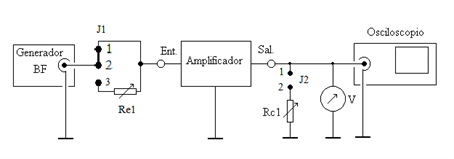
\includegraphics[width=0.9\textwidth]{Imagenes/conexZoLA.png}
    \caption{Conexión del Amplificador de prueba para medir la impedancia de salida}
    \label{fig:conexZoLA}
\end{figure}

El amplificador fue alimentado con una fuente de tensión de 12 V, y la señal de entrada (creada por el generador) tenía una frecuencia de 1 kHz.

Ahora el amplificador se encuentra sin resistencia de carga ($R_{C_1}$), por lo que la tensión que se medirá con el voltímetro y el osciloscopio, será la tensión de salida en vacío. Se procede a variar la tensión de entrada (del generador) hasta justo antes de que la señal de salida se vea recortada (antes de que el amplificador entre en la zona de funcionamiento alineal). Esto se realiza exclusivamente con la finalidad de lograr trabajar con señales más grande para que así sea mas fácil analizarlas y que se vean menos afectadas por el ruido.

La señal de salida $v_s$ máxima que se obtuvo sin recortes fue de 10,2 $V_{pp}$, con una señal de entrada $v_i$ = 3.08 $V_{pp}$.

Sabiendo la tensión de salida en vacío con esa tensión de entrada, se procedió a conectar la carga $R_{C_1}$ (resistor variable), con el jumper $J2$ y se fue variando la resistencia hasta obtener en la salida una señal con la mitad de la amplitud de la señal original. El valor más próximo a este que se obtuvo fue de $v_s'$ = 5,08 $V_{pp}$.

%imagen de la medicion

En esta situación el valor de la impedancia de salida del amplificador es numéricamente igual a la resistencia de carga (debido al tipo de amplificador y la frecuencia en que se hace el ensayo, se puede considerar sin mucho margen de error que la impedancia de salida no tiene parte reactiva considerable), y su valor puede determinarse en forma indirecta midiendo el valor de la resistencia de carga $R_{C_1}$ con un óhmetro. 

Por lo que sin alterar la resistencia, se desconectó el jumper $J2$ para que la medición no se viese afectada por el resto del circuito y se midió la resistencia $R_{C_1}$. En la tabla a continuación se exponen los datos de resistencia recogidos junto con la incertidumbre en la medición (tabla \ref{tab:exp1}).

\subsubsection{Mediciones}

Para la medición de la resistencia se utilizó el multímetro del laboratorio de la marca UNI-T, modelo UT890C, cuyos datos de exactitud, se encuentra en la sección \ref{sec:Información Instrumentos} (Información de Instrumentos), en la tabla \ref{tab:R_UT890C}.

\begin{table}[H]
    \centering
    \scalebox{1}{
    \begin{tabular} {|c|c|c|c|c|}
    %{|m{1.5cm}|m{2.7cm}|m{1cm}|p{1.5cm}|m{2.7cm}|}
   
    \hline
         $f$ & Valor Nominal & $V_s$ & $R_{C_1}=R_o$ & Incertidumbre \\
         
         Frec. Gen. & de $Z_{sal}=R_o$ & en vacío & Para $V_s'=\frac{V_s}{2}$ & medición $R_{C_1}$\\
    \hline
        1 kHz & 50 $\ohm$ & 10.2 $V_{pp}$ & 46.1 $\Omega$ & $\pm$ 0.869 $\Omega$\\
    \hline
        \end{tabular}}
        \def\tablename{Tabla} 
        \caption{Valores esperados y obtenidos}
        \label{tab:exp1}
\end{table}

Afortunadamente, el valor de resistencia obtenido, coincide bastante con el valor esperado para la resistencia de salida. Este es incluso menor, lo que representaría una característica positiva, ya que la impedancia de salida de un amplificador ideal debería ser cero.


%\newpage
\vspace{1.5cm}
\subsection{Experimento 2: Determinación de la impedancia de entrada del amplificador}
\label{sec:exp2}
De manera similar a la sección~\ref{sec:exp1}, en este experimento se nos planteo determinar los valores de los componentes planteados en nuestro modelo para una serie de distintos capacitores. Se redujo la resistencia $R_g$ del circuito anterior debido a que el componente resistivo es menor, dejando la resistencia en $R_g=1~k\Omega$. Se modifico la señal de entrada a una señal cuadrada para facilitar las medición. Ya que, como se explico en la sección~\ref{sec:Cap}, la señal en tensión resultante de este planteamiento sera una señal triangular (debido al efecto integrador de corriente del capacitor) sumada a la misma señal cuadrada (debido al efecto de la resistencia interna del capacitor), se podrá discernir y estimar los distintos componentes a través de la medición la señal a bornes del capacitor.

\begin{figure}[H]
    \centering
    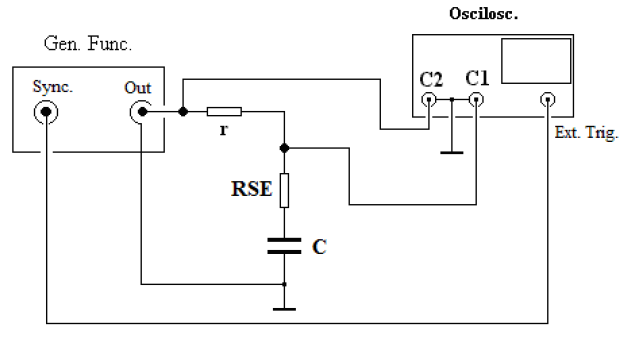
\includegraphics[width=0.7\linewidth]{Imagenes/exp2.png}
    \caption{Circuito experimento 2}
    \label{fig:exp2}
\end{figure}

Según lo anteriormente explicado podemos plantear los siguiente:
\begin{figure}[H]
    \centering
    \begin{minipage}{0.59\textwidth}
        \begin{tikzpicture}[scale=0.65,every node/.style={transform shape}]
\def\res{0.5};%EscalaTemporal señal 1
\def\ind{1};%EscalaTemporal señal 2
\def\scalVa{1};%EscalaVertical señal 1
\def\frec{5};%EscalaVertical señal 2
\def\offseta{0};%Nivel de offset de la señal señal 1
\def\offsetb{};%Nivel de offset de la señal señal 2

%Lineas intermedias grilla
\foreach \x in {-5,-4.8,...,4.8,5}{
    \draw[gray!40,thin,shift={(\x,0)}] (0pt,2pt) -- (0pt,-2pt);
}
\foreach \y in {-4,-3.8,...,3.8,4}{
    \draw[gray!40,thin,shift={(0,\y)}] (2pt,0pt) -- (-2pt,0pt);
}
\foreach \a [evaluate={\y=\a*0.5}] in {-5,-1,1,5}{
    \draw[gray!40,line width=0.7pt,dotted] (-5,\y) -- (5,\y);
}

%Grilla
\draw[thin,gray!40] (-5,-4) grid (5,4);
\node[fill=white,text=gray!40,circle,scale=0.5] at (-5,3) {$100\%$};
\node[fill=white,text=gray!40,circle,scale=0.5] at (-5,2.5) {$90\%$};
\node[fill=white,text=gray!40,circle,scale=0.5] at (-5,-2.5) {$10\%$};
\node[fill=white,text=gray!40,circle,scale=0.5] at (-5,-3) {$0\%$};
\draw[black] (-6,-5) rectangle(6,5);

%Señal 1
\clip (-5,-4) rectangle (5,4);
\foreach [evaluate={\a=\c+2}] \c in{-5,-1,3}{
    \draw[line width=1pt](\c,-2)--(\a,2.5)--(\a,2){};
    \draw[line width=1pt](\a,2)--(\a+2,-2.5)--(\a+2,-2){};
}
\draw[line width=1pt,dashed,stealth-stealth](1,-2.5)--(1,2) node[midway,right]{$v_c$};
\draw[line width=1pt,dashed,stealth-stealth,|-|](-2.8,2)--(-2.8,2.5)node[anchor=north west]{$v_r$};
\end{tikzpicture}
        \label{fig:enter-label}
    \end{minipage}
    \begin{minipage}{0.29\textwidth}
       \begin{circuitikz}[scale=1,every node/.style={transform shape},style=american]
\draw (0,2)to[open,v=$v_i$,o-o](0,-2)--(3,-2)to[capacitor=$C$](3,0)to[R=$r_c$](3,2) (0,2)to[R=$R_g$,i=$i_{(t)}$](3,2);
\draw[line width=0.7pt,dashed] (2.3,-1.8)rectangle(3.3,1.8);
\draw (3.7,0)to[open,v=$v_c$](3.7,-2)  (3.7,2)to[open,v=$v_r$](3.7,0);
\end{circuitikz}

\end{minipage}
\caption{Análisis del circuito equivalente de un capacitor}
\end{figure}
Tomando los valores de los tramos de la señal correspondiente a los distintos componentes, se pude calcular el valor de la resistencia de la siguiente manera:
\begin{equation}
    r_c=\frac{v_r}{i}
\end{equation}

\unsubsubsection{Mediciones}
La señal cuadrada utilizada fue establecida en los siguientes valores: 
\begin{itemize}
    \item $V_{pp}=20~V$
    \item  $F_{rec}=10 ~KHz$
\end{itemize}

Se procedió a medir sobre los puntos establecidos, obteniendo los siguientes datos:
\begin{figure}[H]
    \centering
    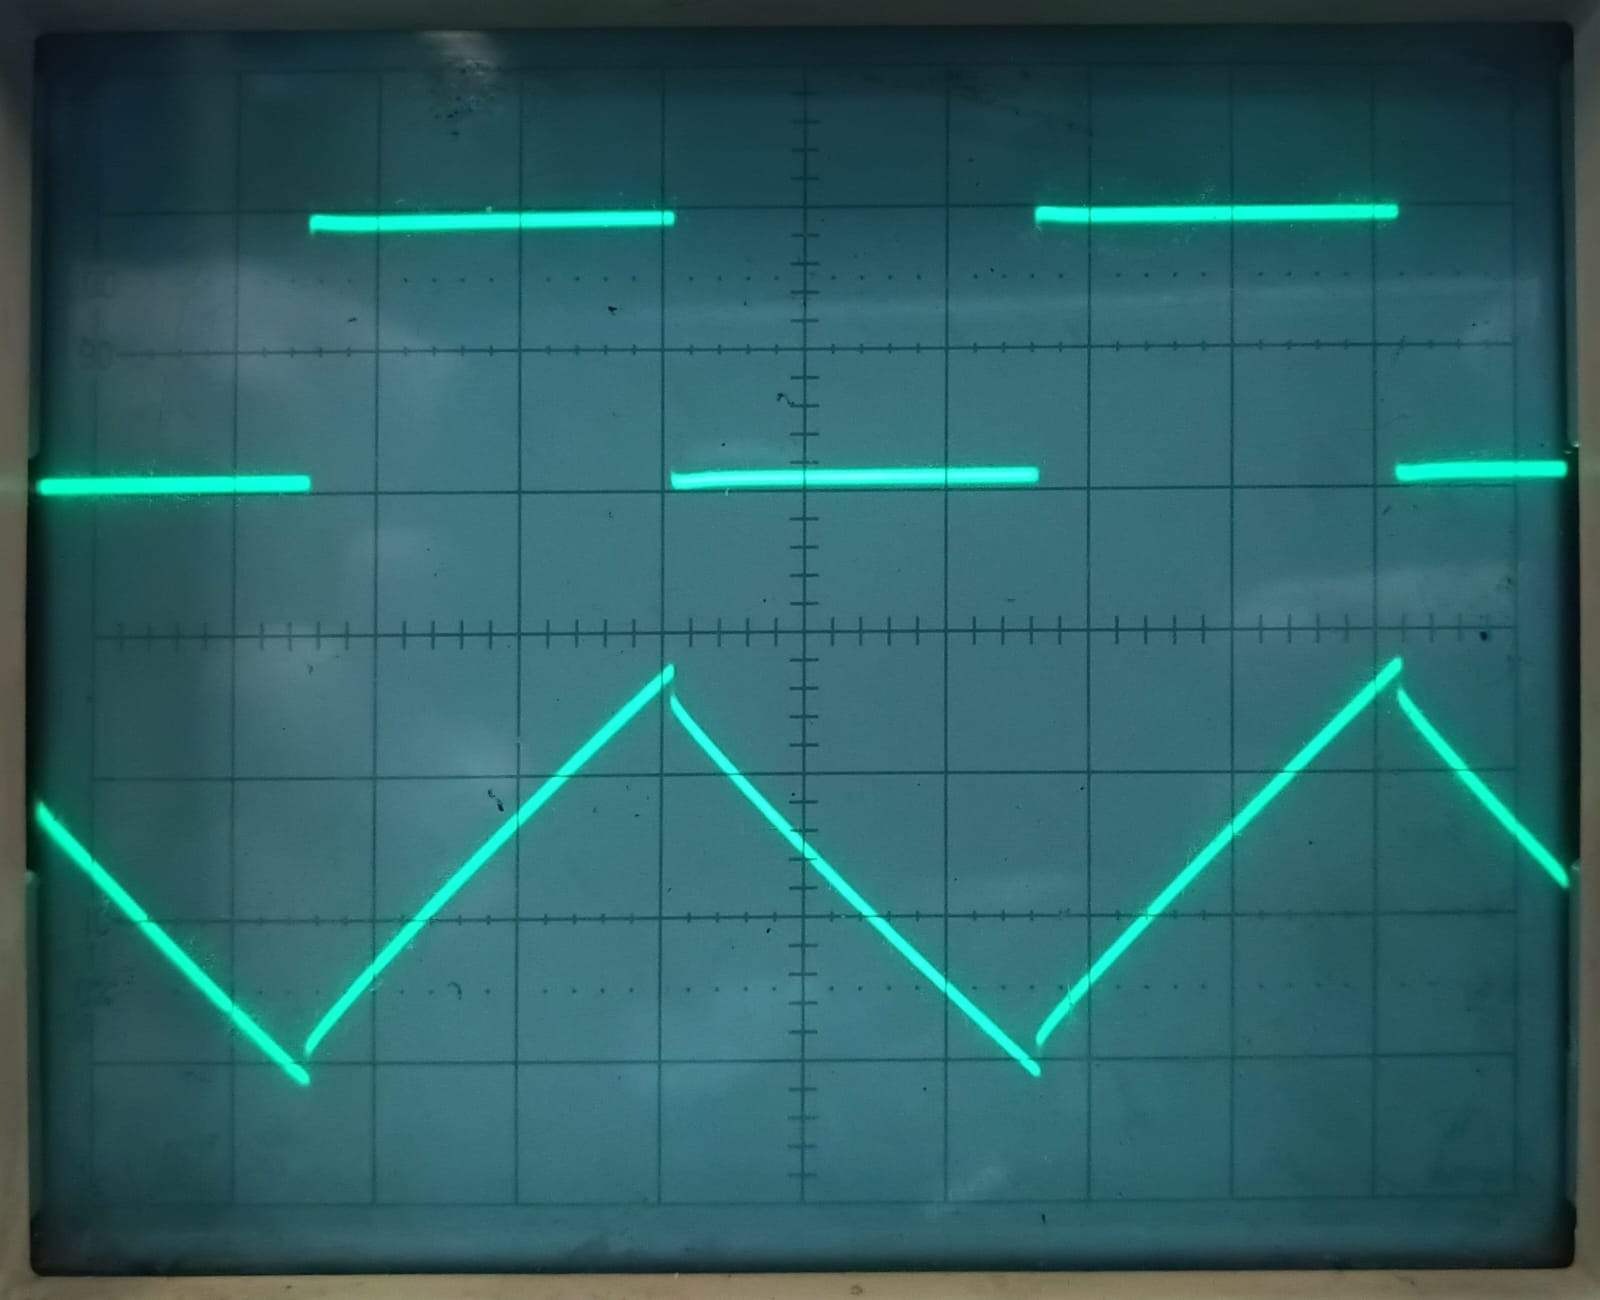
\includegraphics[width=0.6\textwidth]{Imagenes/MedExp2.jpeg}
    \caption{Mediciones de la señal de salida vs entrada del experimento 2}

\end{figure}
\begin{table}[H]
    \centering
    \begin{tabular}{|c|c|c|c|}
    \hline
        $f$ & \multicolumn{3}{c|}{$10~kHz$}\\
    \hline
        $C_{nom}$ & $1~\mu F$ & $2.2~\mu F$ & $4.7~\mu F$ \\ 
    \hline
        $r$ & \multicolumn{3}{c|}{$1~k\Omega$}\\
    \hline
        $e_{pp}~(Canal~2)[V]$ & 20 & 20 & 20\\
    %\hline
        $I=\cfrac{e_{pp}}{r} ~[mA]$ & 18.5 & 18.5 & 18.5 \\
    %\hline    
        $e_R~[mV]$ & 36 & 149.85 & 50 \\
    %\hline    
        $RSE = \cfrac{e_R}{I} ~[\Omega]$ & 1.94 & 7.3 & 2.7 \\
    \hline    
    
        \end{tabular}
        \def\tablename{Tabla} 
        \caption{Tabla de parámetros para distintos capacitores}
        \label{tab:exp2}
\end{table}

\unsubsubsection{Comprobación}
Utilizando un medidor RLC se comprobaron los valores nominales de los 3 capacitores utilizados:

\begin{figure}[H]
\centering
    \begin{minipage}{0.29\textwidth}
    \centering
    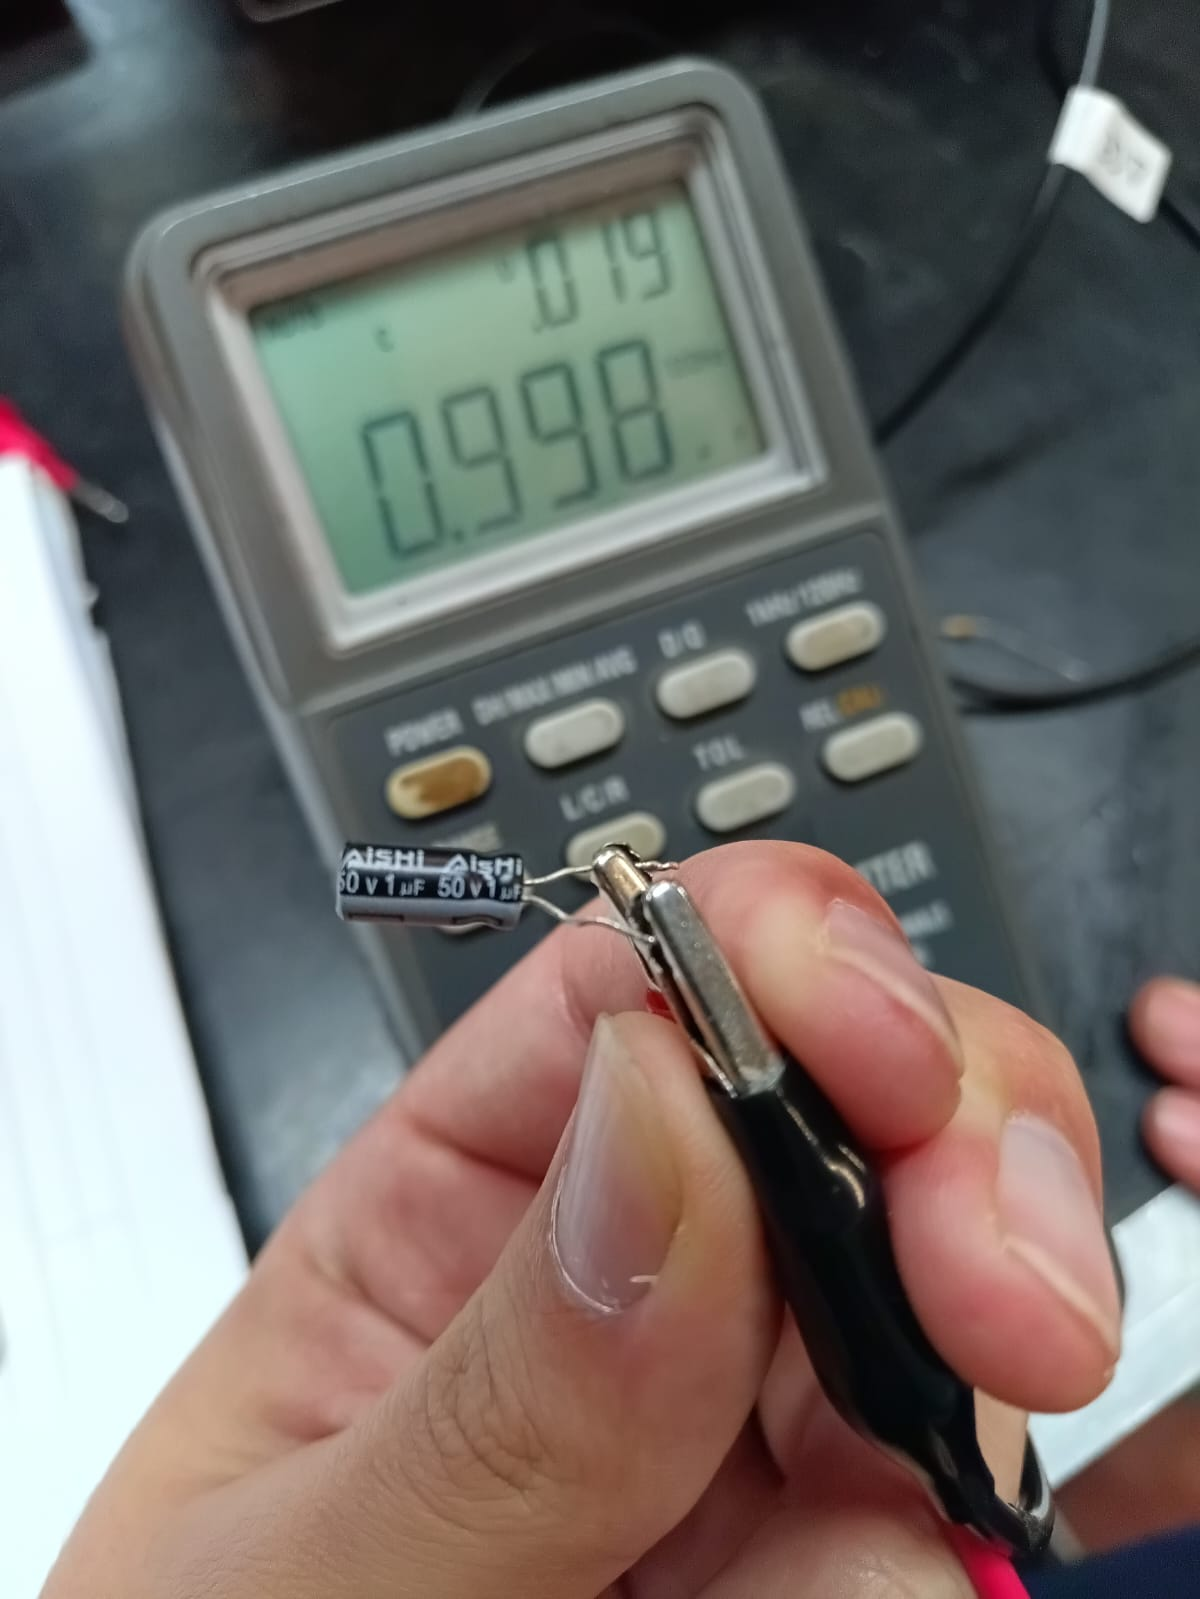
\includegraphics[width=\textwidth,trim={0cm 10cm 0cm 0cm},clip]{Imagenes/MedCap3Exp2.jpeg}
    \caption*{$C=1~\mu F$}
    \end{minipage}
    \hspace*{\fill}
    \begin{minipage}{0.29\textwidth}
    \centering
    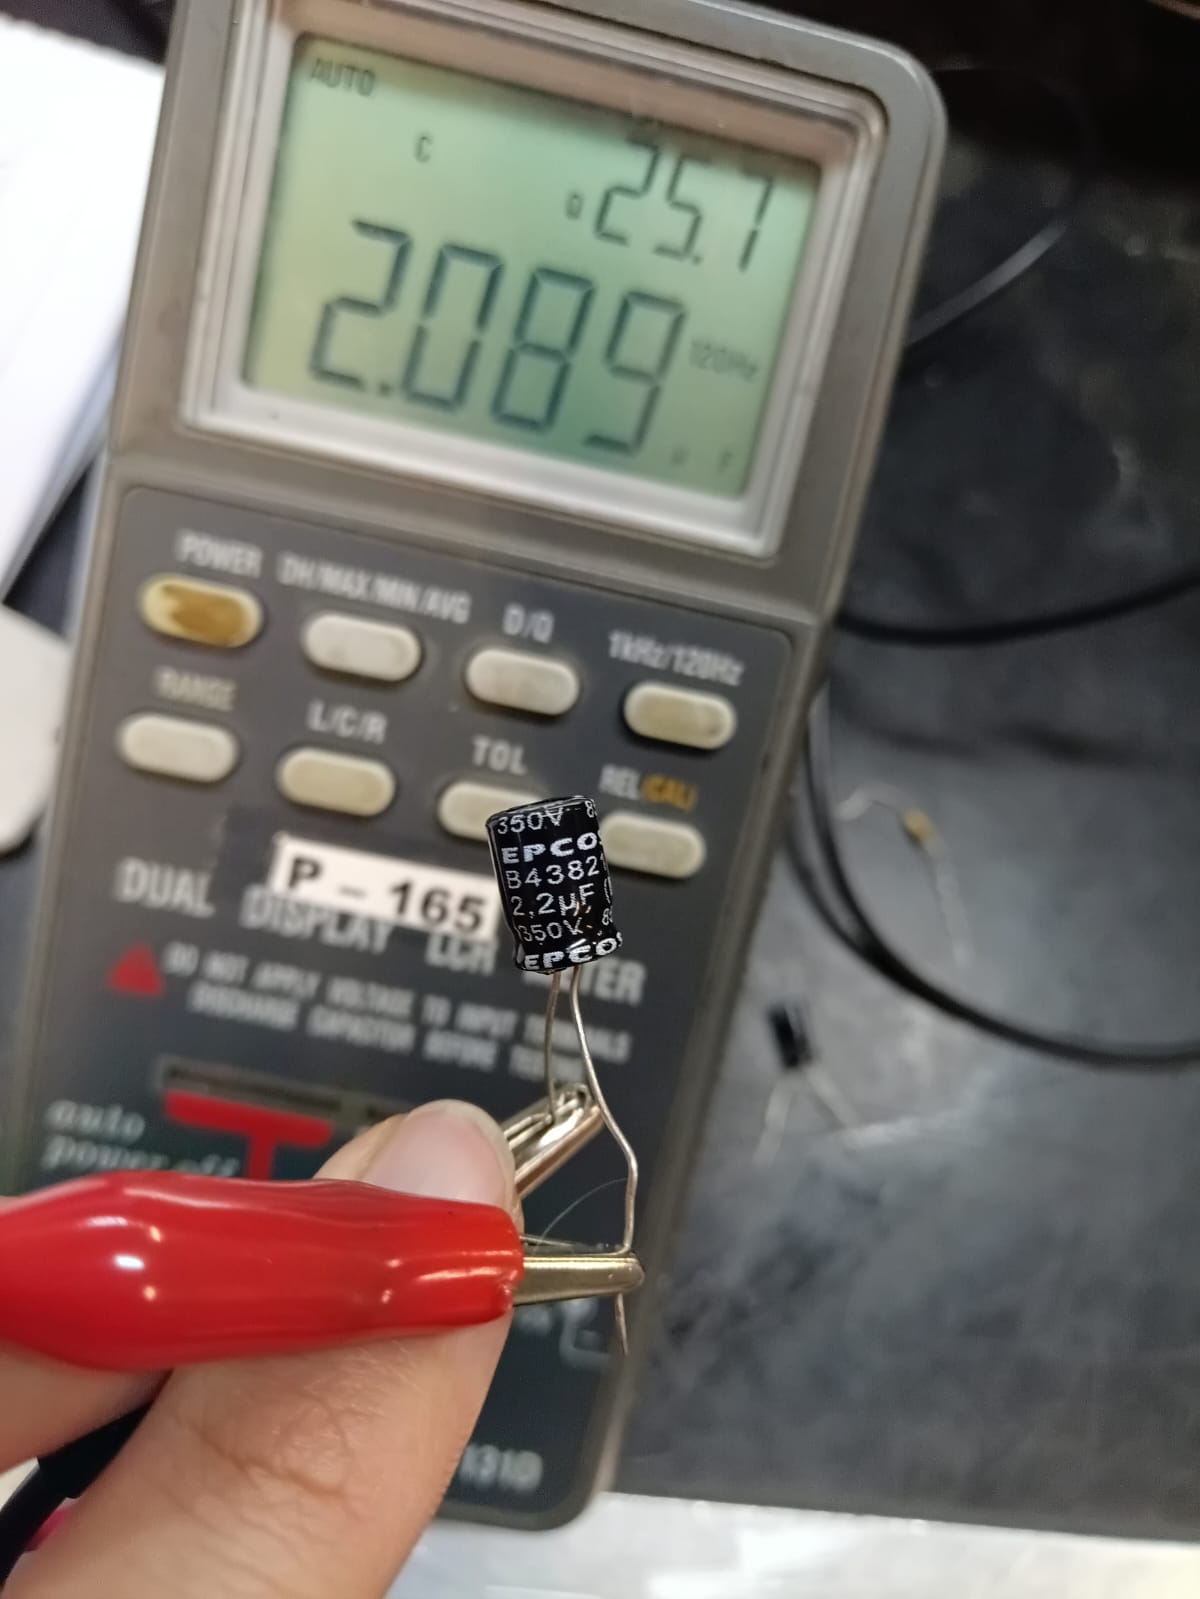
\includegraphics[width=\textwidth,trim={0cm 10cm 0cm 0cm},clip]{Imagenes/MedCap1Exp2.jpeg}
    \caption*{$C=2.2~\mu F$}
    \end{minipage}
    \hspace*{\fill}
    \begin{minipage}{0.29\textwidth}
    \centering
    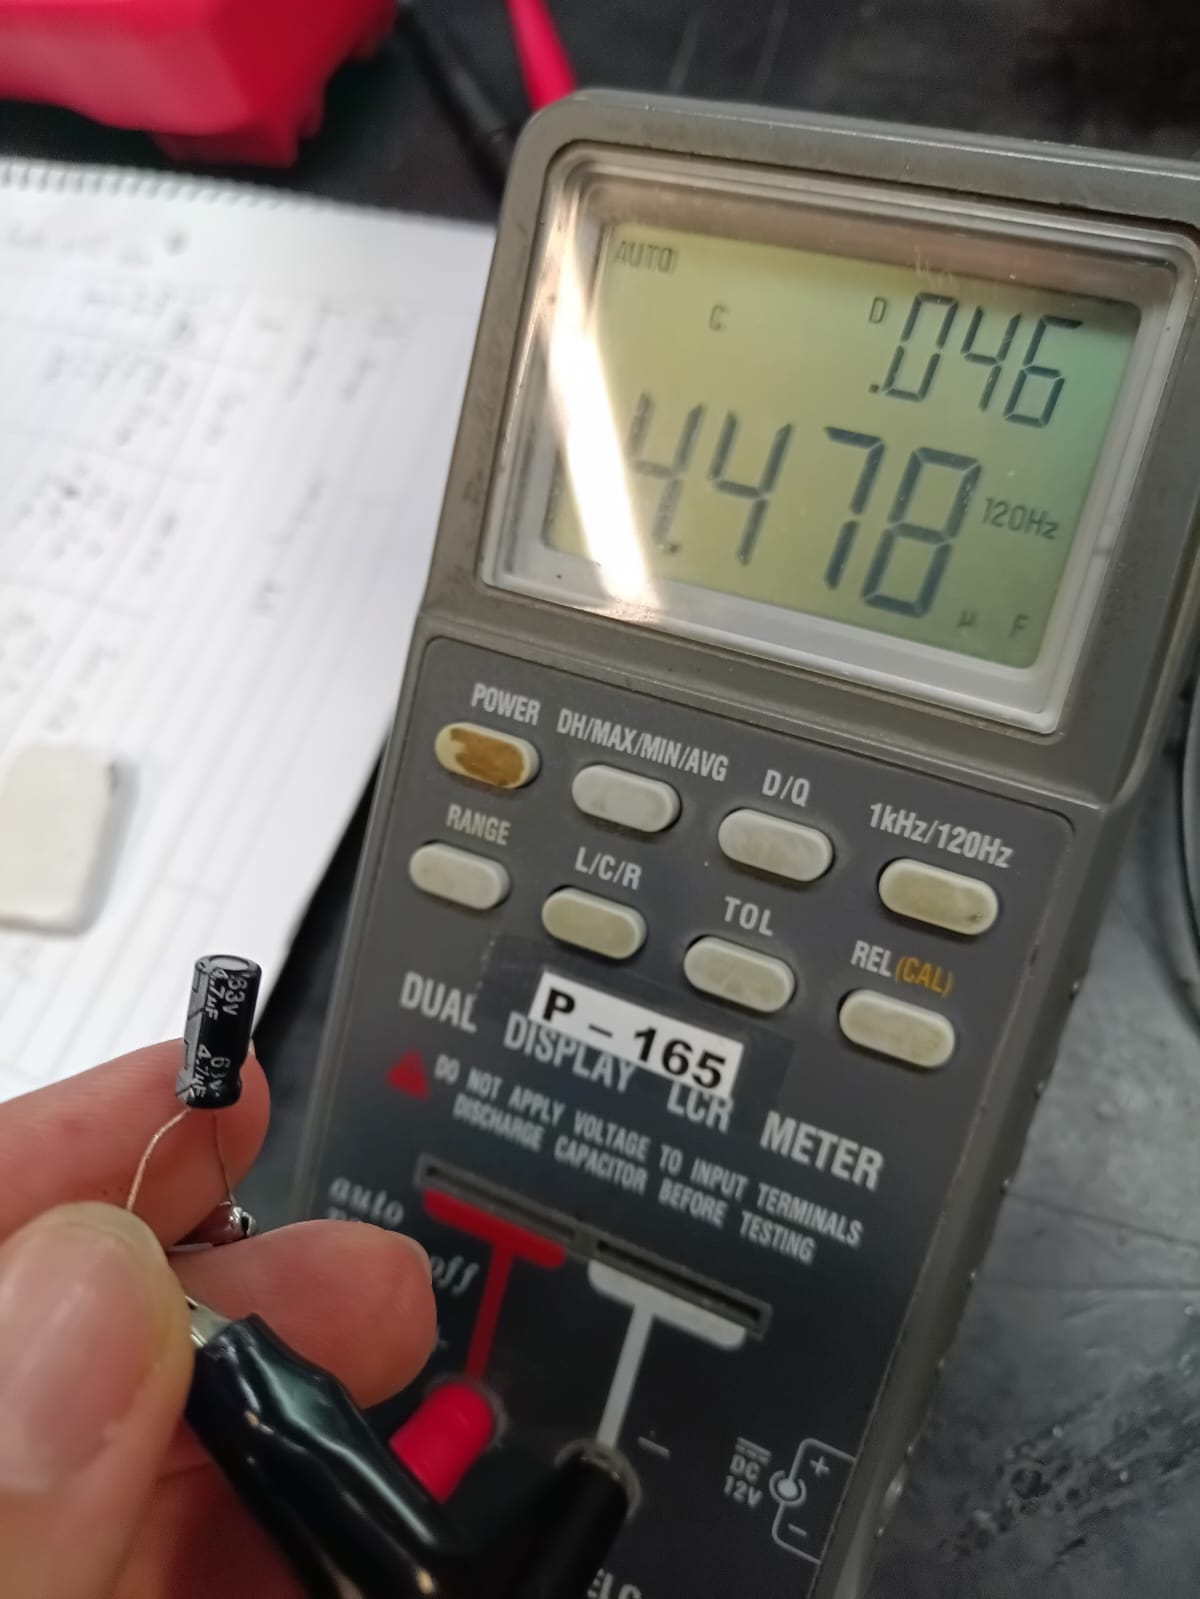
\includegraphics[width=\textwidth,trim={0cm 10cm 0cm 0cm},clip]{Imagenes/MedCap2Exp2.jpeg}
    \caption*{$C=4.7~\mu F$}
    \end{minipage}
    \caption{Mediciones de los capacitores del experimento 2}
\end{figure}

\newpage
\subsection{Experimento 3: Medición de la potencia de salida del amplificador}
Este ensayo se realizó con el objetivo de medir la potencia de salida del amplificador utilizado en los dos puntos anteriores. La potencia fue medida para las condiciones de resistencia de carga igual a la impedancia de salida y máxima excursión simétrica de la tensión de salida. Ver fundamentos de este experimento en la sección \ref{sec:MaxPot}, del Marco Teórico.

Una de las formas más comunes de expresar el valor de la potencia de salida de un amplificador es en \textbf{dBm}, el cual es una unidad de medida de relación o razón de potencia expresada en decibelios con referencia a 1mW. Se puede obtener su valor a partir de la expresión \ref{eq::PotConVolReferidoa775mV} (Marco Teórico).

La forma más sencilla de determinar la \textbf{dBm} es mediante el empleo de instrumentos que posean escalas trazadas en \textbf{dB}, como lo es el multímetro analógico de la marca UNIVO.
Este instrumento no tiene la funcionalidad de medir potencia, pero se la puede medir indirectamente a partir de la medición de la tensión en la carga $R_{C1}$ en escala de decibeles. Como se explicó en el apartado \ref{sec:Gan} del marco teórico, por lo general la tensión se mide en la unidad de \textbf{dBu} (decibelios referidos a 0.775V).

Para esto, se dispuso los instrumentos de la misma forma que en la experiencia 1, conectando la carga $R_{C1}$ y moviendo la perilla hasta lograr el valor de resistencia igual a la impedancia de salida, el cual es de $ Z_o = 46.1 \pm 0.869  ~\Omega$.

Lo siguiente fue configurar el multímetro en la escala de decibeles, que está trazada
en el rango de 3V, y se procedió a conectar los terminales del multímetro a una tensión fija de 0.775V para poder calibrar el punto de 0 decibelios. 

\subsubsection{Mediciones}

Una vez terminada la calibración, se conectaron los terminales en paralelo con la resistencia de carga $R_{C1}$ para medir la caída de tensión. Para esta medición, el voltímetro estaba configurado para medir corriente alterna y además las puntas estaban conectadas una al borne común del multímetro y la otra a la terminal OUTPUT.

El resultado de la medición se visualiza en la figura \ref{fig:VoltajeDeSalidaDBu}.

\begin{equation}
    V_{dBu} = 8.20 \mathrm{dBu}
\end{equation}


\begin{figure}[H]
    \centering
    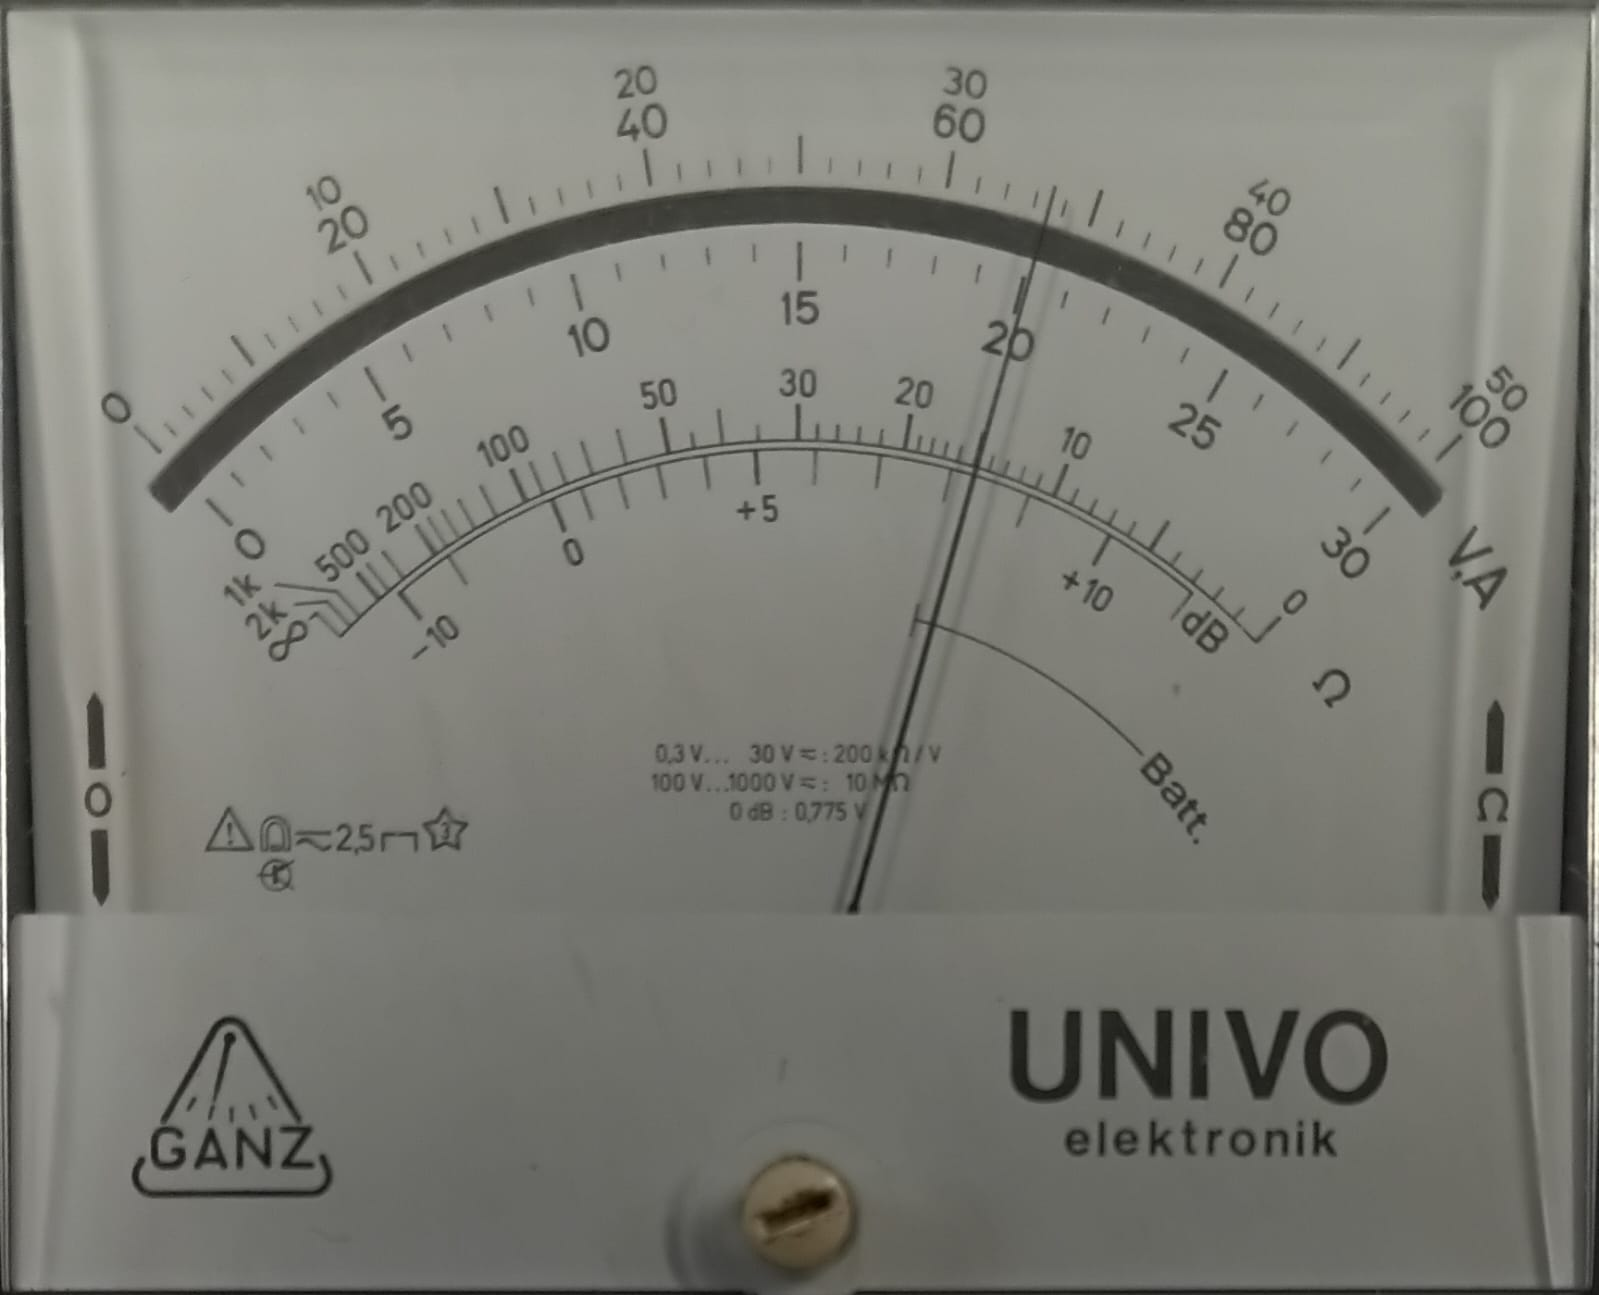
\includegraphics[width=0.45\linewidth]{Imagenes/dBuSal.jpeg}
    \caption{Voltaje de Salida en dBu}
    \label{fig:VoltajeDeSalidaDBu}
\end{figure}

Este valor en dBu obtenido es el primer término de la ecuación \ref{eq::PotConVolReferidoa775mV}, al cual se le debe sumar el término correspondiente a la resistencia sobre la que se midió ese voltaje. Por lo tanto, usando la ecuación, se obtiene que:

\begin{equation}
    P_{dBm} = V_{dBu} + 10\cdot\log{\frac{600\Omega}{R_x}}
\end{equation}

Reemplazando $V_{dBu}$ por el valor medido, y $R_x$ por la resistencia $R_{C1}$ sobre la cual se midió:

\begin{align}
    P_{dBm} =& 8.20 \mathrm{dB} + 10\cdot\log{\frac{600\Omega}{46.1\Omega}}
    \\ =& 8.20 \mathrm{dB} + 11.14 \mathrm{dB}
    \\ =& 19.34 \mathrm{dB}
\end{align}

\subsubsection{Comprobación}

Se puede comprobar la exactitud de este valor, calculando la potencia sobre la resistencia de salida y luego haciendo la conversión a \textit{dBm}. 

Para realizar este cálculo, tomaremos algunos datos del experimento 1: 

\begin{align*}
    v_s = 10,2 V_{pp} = 5,1 V_p
    \hspace{0.5cm}\longrightarrow \hspace{0.5cm}\text{En vacío}\\
    v_s'= 5,08 V_{pp} = 2,54 V_p 
    \hspace{0.5cm}\longrightarrow \hspace{0.5cm}\text{Con} ~R_{cl}=Z_o
\end{align*}

Ahora, se calculará la corriente eficaz $I_{ef}$ que circula por la resistencia $R_{cl}$.

\begin{equation*}
    I_{ef} = \cfrac{\cfrac{v_s}{\sqrt{2}}}{2 \cdot Z_o} 
    = \cfrac{\cfrac{2.54}{\sqrt{2}}}{2 \cdot 46.1} = 39.113 mA
    %\hspace{0.5cm} \Longrightarrow \hspace{0.5cm}
\end{equation*}

Entonces la potencia sobre la resistencia de carga en la salida será:

\begin{equation*}
    P = I_{ef} \cdot V_{ef}' = I_{ef} \cdot \cfrac{v_s'}{\sqrt{2}}
    = 39.113 \cdot 10^{-3} \cdot \cfrac{2.54}{\sqrt{2}} = 70.25 mW
\end{equation*}

Finalmente convertimos a dBm y comparamos resultados.

\begin{equation*}
    P_{dBm} = 10 \cdot \log \left( \cfrac{P}{1 mW} \right) = 10 \cdot \log \left( \cfrac{70.25 mW}{1 mW} \right) = 18.466 ~dBm
\end{equation*}

A primera vista parece un valor muy similar al obtenido en la medición, sin embargo cuando se transforma a mW el valor en dBm de la medición, se obtiene un valor de 85.9 mW, que está bastante alejado del valor calculado. 

Esta diferencia entre cálculo y medición, puede deberse a fallas en la calibración del instrumento para medir potencia y/o por falta de exactitud de este.


\newpage
\subsection{Experimento 4: Medición de la ganancia de tensión y ganancia de potencia del amplificador}
Continuando con el análisis de las mediciones de un multimetro true RMS, en este experimento se busca comparar nuevamente los valores dados por este multimetro en comparación con uno que brinda el valor medio de la señal, para ello se procedió a medir la forma de onda proveniente de un circuito con control de ángulo de conducción, el cual se puede observar en la figura \ref{fig:circ_triac}




\begin{figure}[H]
    \centering
    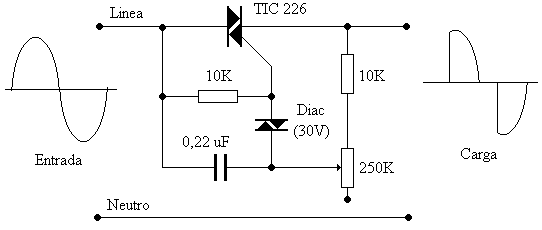
\includegraphics[width=0.8\linewidth]{Imagenes/circ_triac.png}
    \caption{Circuito Experimento 4: Control de ángulo de conducción}
    \label{fig:circ_triac}
\end{figure}

Este circuito se conecto a la tensión de linea y se procedió a conectar los multimetros y el osciloscopio, utilizando siempre el transformador de aislación para evitar inconvenientes que causen daños a los instrumentos. En la figura \ref{fig:conec_exp4}se observa la conexión correcta para realizar la experimentación. 
\begin{figure}[H]
    \centering
    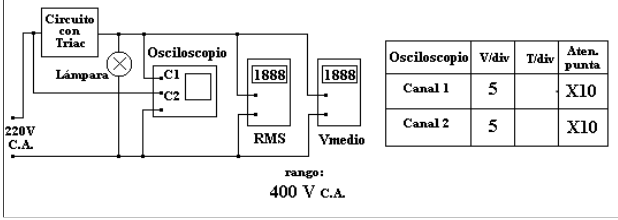
\includegraphics[width=0.6\linewidth,trim= 5pt 5pt 8.5cm 0,clip]{Imagenes/conec_exp4.png}
    \caption{Conexión Experimento 4}
    \label{fig:conec_exp4}
\end{figure}

\begin{table}[H]
    \centering
    \scalebox{1}{
    \begin{tabular}{|c|c|c|c|c|}
    \hline
         V/div (C. Y1) & V/div (C.Y2) & t/div & Aten. Y1 & Aten. Y2 \\
    \hline
         5 $V$ & 5 $V$ &  $ms$ & x10 & x10\\
    \hline
    \end{tabular}}
        %\def\tablename{Tabla} 
        \caption{Configuración del Osciloscopio}
        \label{tab:cont4}
\end{table}
Como primer paso se midió la tensión de entrada al circuito, obteniendo el siguiente valor.

\begin{equation*}
    V_i = 230.8 ~[V]
\end{equation*}

Luego a través del potenciómetro que viene incluido en el circuito de control, se fue variando el ángulo de conducción y a su vez se fue midiendo los valores de tensión que había a la salida del circuito. Se variaron los ángulos de salida según las siguientes gráficas, y se espera obtener formas de onda similares en las mediciones.

\begin{figure}[H]
    \centering
    \begin{minipage}{0.49\textwidth}
        \centering
        \begin{tikzpicture}[scale=0.5,every node/.style={transform shape}]
\def\angC{180}
    %Lineas intermedias grilla
    \foreach \x in {-5,-4.8,...,4.8,5}{
        \draw[gray!40,thin,shift={(\x,0)}] (0pt,2pt) -- (0pt,-2pt);
    }
    \foreach \y in {-4,-3.8,...,3.8,4}{
        \draw[gray!40,thin,shift={(0,\y)}] (2pt,0pt) -- (-2pt,0pt);
    }
    \foreach \a [evaluate={\y=\a*0.5}] in {-5,-1,1,5}{
        \draw[gray!40,line width=0.7pt,dotted] (-5,\y) -- (5,\y);
    }

    %Grilla
    \draw[thin,gray!40] (-5,-4) grid (5,4);
    \node[fill=white,text=gray!40,circle,scale=0.5] at (-5,3) {$100\%$};
    \node[fill=white,text=gray!40,circle,scale=0.5] at (-5,2.5) {$90\%$};
    \node[fill=white,text=gray!40,circle,scale=0.5] at (-5,-2.5) {$10\%$};
    \node[fill=white,text=gray!40,circle,scale=0.5] at (-5,-3) {$0\%$};
    \draw[black] (-6,-5) rectangle(6,5);
    
    
    \draw [line width=1pt,black] plot[smooth,samples=100,domain=-5:5](\x,{2*sin(deg(\x*pi*0.2))+2});

    
    \draw [thin,black] plot[smooth,samples=100,domain=\angC/36:5](\x,{2*sin(deg(\x*pi*0.2))-2});
    \draw [thin,black] plot[smooth,samples=100,domain=-5+\angC/36:0](\x,{2*sin(deg(\x*pi*0.2))-2});
    \draw[thin,black](\angC/36,{2*sin(deg(3.14*\angC/36*0.2))-2})--(\angC/36,-2);
    \draw[thin,black](-5+\angC/36,{2*sin(deg(3.14*(-5+\angC/36)*0.2))-2})--(-5+\angC/36,-2);
    \draw[line width=1pt,black](-5,-2)--(-5+\angC/36,-2) (0,-2)--(\angC/36,-2);
\end{tikzpicture}
\caption*{$Ang_{cond}=0$}
    \end{minipage}
    \begin{minipage}{0.49\textwidth}
        \centering
        \begin{tikzpicture}[scale=0.5,every node/.style={transform shape}]
\def\angC{150}
    %Lineas intermedias grilla
    \foreach \x in {-5,-4.8,...,4.8,5}{
        \draw[gray!40,thin,shift={(\x,0)}] (0pt,2pt) -- (0pt,-2pt);
    }
    \foreach \y in {-4,-3.8,...,3.8,4}{
        \draw[gray!40,thin,shift={(0,\y)}] (2pt,0pt) -- (-2pt,0pt);
    }
    \foreach \a [evaluate={\y=\a*0.5}] in {-5,-1,1,5}{
        \draw[gray!40,line width=0.7pt,dotted] (-5,\y) -- (5,\y);
    }

    %Grilla
    \draw[thin,gray!40] (-5,-4) grid (5,4);
    \node[fill=white,text=gray!40,circle,scale=0.5] at (-5,3) {$100\%$};
    \node[fill=white,text=gray!40,circle,scale=0.5] at (-5,2.5) {$90\%$};
    \node[fill=white,text=gray!40,circle,scale=0.5] at (-5,-2.5) {$10\%$};
    \node[fill=white,text=gray!40,circle,scale=0.5] at (-5,-3) {$0\%$};
    \draw[black] (-6,-5) rectangle(6,5);
    
    
    \draw [line width=1pt,black] plot[smooth,samples=100,domain=-5:5](\x,{2*sin(deg(\x*pi*0.2))+2});

    \draw [thin,black] plot[smooth,samples=100,domain=\angC/36:5](\x,{2*sin(deg(\x*pi*0.2))-2});
    \draw [thin,black] plot[smooth,samples=100,domain=-5+\angC/36:0](\x,{2*sin(deg(\x*pi*0.2))-2});
    \draw[thin,black](\angC/36,{2*sin(deg(3.14*\angC/36*0.2))-2})--(\angC/36,-2);
    \draw[thin,black](-5+\angC/36,{2*sin(deg(3.14*(-5+\angC/36)*0.2))-2})--(-5+\angC/36,-2);
    \draw[line width=1pt,black](-5,-2)--(-5+\angC/36,-2) (0,-2)--(\angC/36,-2);
\end{tikzpicture}
\caption*{$Ang_{cond}=30$}
    \end{minipage}
    \begin{minipage}{0.49\textwidth}
        \centering
        \begin{tikzpicture}[scale=0.5,every node/.style={transform shape}]
\def\angC{120}
    %Lineas intermedias grilla
    \foreach \x in {-5,-4.8,...,4.8,5}{
        \draw[gray!40,thin,shift={(\x,0)}] (0pt,2pt) -- (0pt,-2pt);
    }
    \foreach \y in {-4,-3.8,...,3.8,4}{
        \draw[gray!40,thin,shift={(0,\y)}] (2pt,0pt) -- (-2pt,0pt);
    }
    \foreach \a [evaluate={\y=\a*0.5}] in {-5,-1,1,5}{
        \draw[gray!40,line width=0.7pt,dotted] (-5,\y) -- (5,\y);
    }

    %Grilla
    \draw[thin,gray!40] (-5,-4) grid (5,4);
    \node[fill=white,text=gray!40,circle,scale=0.5] at (-5,3) {$100\%$};
    \node[fill=white,text=gray!40,circle,scale=0.5] at (-5,2.5) {$90\%$};
    \node[fill=white,text=gray!40,circle,scale=0.5] at (-5,-2.5) {$10\%$};
    \node[fill=white,text=gray!40,circle,scale=0.5] at (-5,-3) {$0\%$};
    \draw[black] (-6,-5) rectangle(6,5);
    
    
    \draw [line width=1pt,black] plot[smooth,samples=100,domain=-5:5](\x,{2*sin(deg(\x*pi*0.2))+2});

   
    \draw [thin,black] plot[smooth,samples=100,domain=\angC/36:5](\x,{2*sin(deg(\x*pi*0.2))-2});
    \draw [thin,black] plot[smooth,samples=100,domain=-5+\angC/36:0](\x,{2*sin(deg(\x*pi*0.2))-2});
    \draw[thin,black](\angC/36,{2*sin(deg(3.14*\angC/36*0.2))-2})--(\angC/36,-2);
    \draw[thin,black](-5+\angC/36,{2*sin(deg(3.14*(-5+\angC/36)*0.2))-2})--(-5+\angC/36,-2);
    \draw[line width=1pt,black](-5,-2)--(-5+\angC/36,-2) (0,-2)--(\angC/36,-2);
\end{tikzpicture}
\caption*{$Ang_{cond}=60$}
    \end{minipage}
    \centering
    \begin{minipage}{0.49\textwidth}
    \centering
        \begin{tikzpicture}[scale=0.5,every node/.style={transform shape}]
\def\angC{90}
    %Lineas intermedias grilla
    \foreach \x in {-5,-4.8,...,4.8,5}{
        \draw[gray!40,thin,shift={(\x,0)}] (0pt,2pt) -- (0pt,-2pt);
    }
    \foreach \y in {-4,-3.8,...,3.8,4}{
        \draw[gray!40,thin,shift={(0,\y)}] (2pt,0pt) -- (-2pt,0pt);
    }
    \foreach \a [evaluate={\y=\a*0.5}] in {-5,-1,1,5}{
        \draw[gray!40,line width=0.7pt,dotted] (-5,\y) -- (5,\y);
    }

    %Grilla
    \draw[thin,gray!40] (-5,-4) grid (5,4);
    \node[fill=white,text=gray!40,circle,scale=0.5] at (-5,3) {$100\%$};
    \node[fill=white,text=gray!40,circle,scale=0.5] at (-5,2.5) {$90\%$};
    \node[fill=white,text=gray!40,circle,scale=0.5] at (-5,-2.5) {$10\%$};
    \node[fill=white,text=gray!40,circle,scale=0.5] at (-5,-3) {$0\%$};
    \draw[black] (-6,-5) rectangle(6,5);
    
    
    \draw [line width=1pt,black] plot[smooth,samples=100,domain=-5:5](\x,{2*sin(deg(\x*pi*0.2))+2});

    \draw [thin,black] plot[smooth,samples=100,domain=\angC/36:5](\x,{2*sin(deg(\x*pi*0.2))-2});
    \draw [thin,black] plot[smooth,samples=100,domain=-5+\angC/36:0](\x,{2*sin(deg(\x*pi*0.2))-2});
    \draw[thin,black](\angC/36,{2*sin(deg(3.14*\angC/36*0.2))-2})--(\angC/36,-2);
    \draw[thin,black](-5+\angC/36,{2*sin(deg(3.14*(-5+\angC/36)*0.2))-2})--(-5+\angC/36,-2);
    \draw[line width=1pt,black](-5,-2)--(-5+\angC/36,-2) (0,-2)--(\angC/36,-2);
\end{tikzpicture}
\caption*{$Ang_{cond}=90$}
    \end{minipage}
    \begin{minipage}{0.49\textwidth}
    \centering
        \begin{tikzpicture}[scale=0.5,every node/.style={transform shape}]
\def\angC{60}
    %Lineas intermedias grilla
    \foreach \x in {-5,-4.8,...,4.8,5}{
        \draw[gray!40,thin,shift={(\x,0)}] (0pt,2pt) -- (0pt,-2pt);
    }
    \foreach \y in {-4,-3.8,...,3.8,4}{
        \draw[gray!40,thin,shift={(0,\y)}] (2pt,0pt) -- (-2pt,0pt);
    }
    \foreach \a [evaluate={\y=\a*0.5}] in {-5,-1,1,5}{
        \draw[gray!40,line width=0.7pt,dotted] (-5,\y) -- (5,\y);
    }

    %Grilla
    \draw[thin,gray!40] (-5,-4) grid (5,4);
    \node[fill=white,text=gray!40,circle,scale=0.5] at (-5,3) {$100\%$};
    \node[fill=white,text=gray!40,circle,scale=0.5] at (-5,2.5) {$90\%$};
    \node[fill=white,text=gray!40,circle,scale=0.5] at (-5,-2.5) {$10\%$};
    \node[fill=white,text=gray!40,circle,scale=0.5] at (-5,-3) {$0\%$};
    \draw[black] (-6,-5) rectangle(6,5);
    
    
    \draw [line width=1pt,black] plot[smooth,samples=100,domain=-5:5](\x,{2*sin(deg(\x*pi*0.2))+2});

    \draw [thin,black] plot[smooth,samples=100,domain=\angC/36:5](\x,{2*sin(deg(\x*pi*0.2))-2});
    \draw [thin,black] plot[smooth,samples=100,domain=-5+\angC/36:0](\x,{2*sin(deg(\x*pi*0.2))-2});
    \draw[thin,black](\angC/36,{2*sin(deg(3.14*\angC/36*0.2))-2})--(\angC/36,-2);
    \draw[thin,black](-5+\angC/36,{2*sin(deg(3.14*(-5+\angC/36)*0.2))-2})--(-5+\angC/36,-2);
    \draw[line width=1pt,black](-5,-2)--(-5+\angC/36,-2) (0,-2)--(\angC/36,-2);
\end{tikzpicture}
\caption*{$Ang_{cond}=120$}
    \end{minipage}
    \begin{minipage}{0.49\textwidth}
    \centering
        \begin{tikzpicture}[scale=0.5,every node/.style={transform shape}]
\def\angC{30}
    %Lineas intermedias grilla
    \foreach \x in {-5,-4.8,...,4.8,5}{
        \draw[gray!40,thin,shift={(\x,0)}] (0pt,2pt) -- (0pt,-2pt);
    }
    \foreach \y in {-4,-3.8,...,3.8,4}{
        \draw[gray!40,thin,shift={(0,\y)}] (2pt,0pt) -- (-2pt,0pt);
    }
    \foreach \a [evaluate={\y=\a*0.5}] in {-5,-1,1,5}{
        \draw[gray!40,line width=0.7pt,dotted] (-5,\y) -- (5,\y);
    }

    %Grilla
    \draw[thin,gray!40] (-5,-4) grid (5,4);
    \node[fill=white,text=gray!40,circle,scale=0.5] at (-5,3) {$100\%$};
    \node[fill=white,text=gray!40,circle,scale=0.5] at (-5,2.5) {$90\%$};
    \node[fill=white,text=gray!40,circle,scale=0.5] at (-5,-2.5) {$10\%$};
    \node[fill=white,text=gray!40,circle,scale=0.5] at (-5,-3) {$0\%$};
    \draw[black] (-6,-5) rectangle(6,5);
    
    
    \draw [line width=1pt,black] plot[smooth,samples=100,domain=-5:5](\x,{2*sin(deg(\x*pi*0.2))+2});

    \draw [thin,black] plot[smooth,samples=100,domain=\angC/36:5](\x,{2*sin(deg(\x*pi*0.2))-2});
    \draw [thin,black] plot[smooth,samples=100,domain=-5+\angC/36:0](\x,{2*sin(deg(\x*pi*0.2))-2});
    \draw[thin,black](\angC/36,{2*sin(deg(3.14*\angC/36*0.2))-2})--(\angC/36,-2);
    \draw[thin,black](-5+\angC/36,{2*sin(deg(3.14*(-5+\angC/36)*0.2))-2})--(-5+\angC/36,-2);
    \draw[line width=1pt,black](-5,-2)--(-5+\angC/36,-2) (0,-2)--(\angC/36,-2);
\end{tikzpicture}
\caption*{$Ang_{cond}=150$}
    \end{minipage}
\end{figure}


\unsubsubsection{Mediciones}

Estas mediciones fueron realizadas con los dos multímetros al mismo tiempo para así ir visualizando la diferencia entre los que media uno y lo que media el otro, obteniendo así la siguiente tabla de comparación.

\begin{table}[H]
    \centering
    \begin{tabular}{|c|c|c|c|c|c|c|c|}
    \hline
        \multirow{2}{*}{Fase} & $V_o$ (1) & $V_o$ (2) & \multirow{2}{*}{$\cfrac{V_{o_1}}{V_i}$} & \multirow{2}{*}{$\cfrac{V_{o_2}}{V_i}$} & Incertidumbre & Incertidumbre&Factor de\\
         & [V] & [V] &  &  & medición $V_{o_1}$ & medición $V_{o_2}$& corrección $\kappa$\\
        \hline
        0° & 0 & 0 & 0 & 0 & $\pm$0 & $\pm$0&0 \\ \hline
        30° & 43 & 17 & 0.186 & 0.074 & $\pm$0.37 & $\pm$0.51& 2.52 \\ \hline
        60° & 89 & 47 & 0.386 & 0.204 & $\pm$1.01 & $\pm$0.864&1.89 \\ \hline
        90° & 116 & 68 & 0.503 & 0.295 & $\pm$1.23 & $\pm$1.12& 1.70\\ \hline
        120° & 209 & 177 & 0.906 & 0.767 & $\pm$1.97 & $\pm$5.12& 1.18\\ \hline
        150° & 227 & 215 & 0.984 & 0.931 & $\pm$2.12 & $\pm$5.58& 1.05\\ \hline
        180° & 231 & 231 & 1 & 1 & $\pm$2.14 & $\pm$5.76& 1\\ \hline
    \end{tabular}
    \def\tablename{Tabla} 
    \caption{mediciones obtenidas}
    \label{tab:exp4}
\end{table}

A continuación en la figura \ref{fig:fot_exp4} se muestran las imágenes las formas de ondas visualizadas en el osciloscopio. Para poder observar dichas ondas completas en la pantalla fue necesario utilizar vernier de ganancia al máximo para atenuar las señales a un 30\% de su valor original.

\begin{figure}[H]
    \begin{center}
        \begin{subfigure}[b]{0.5\textwidth}
        \centering  
            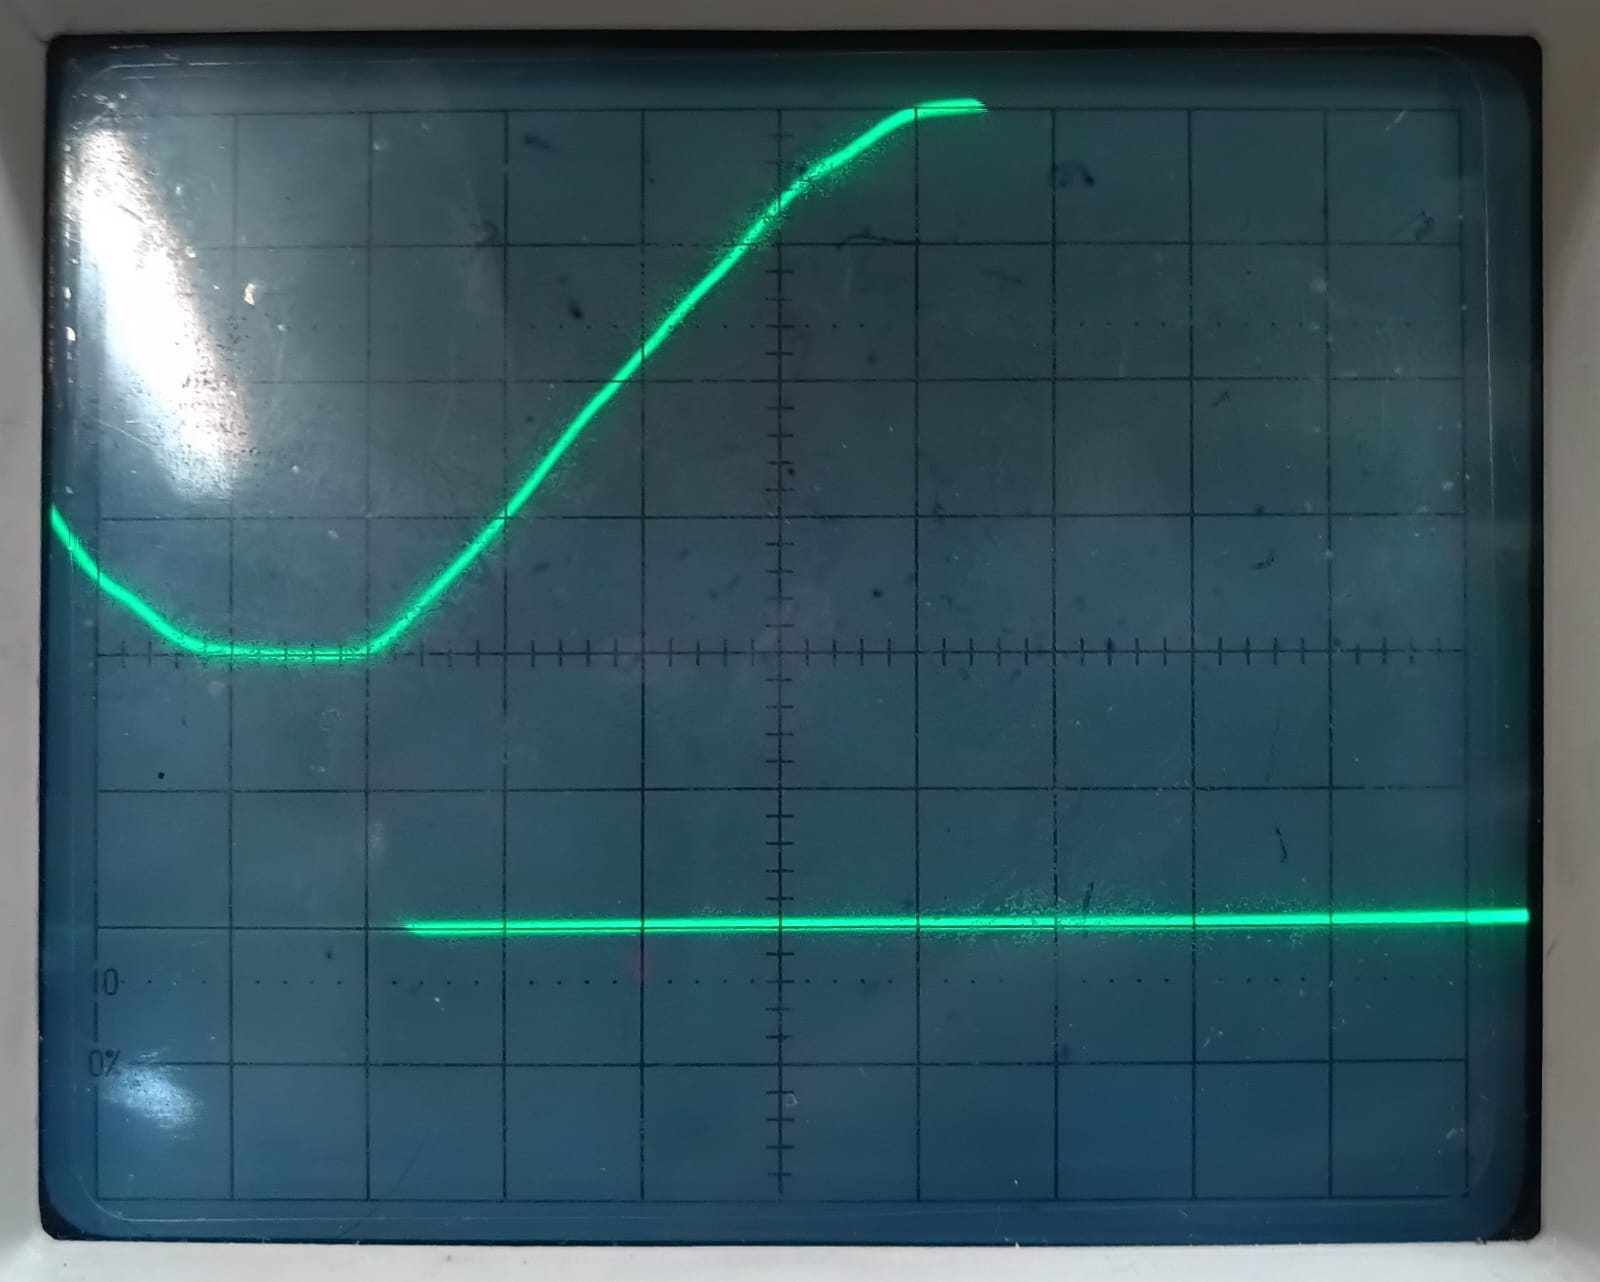
\includegraphics[width=0.65\textwidth]{Imagenes/0grad.jpeg}
        \label{}
        \caption{$Ang_{cond}=0$°}
    \end{subfigure}
    \hfill
        \begin{subfigure}[b]{0.49\textwidth}
        \centering  
            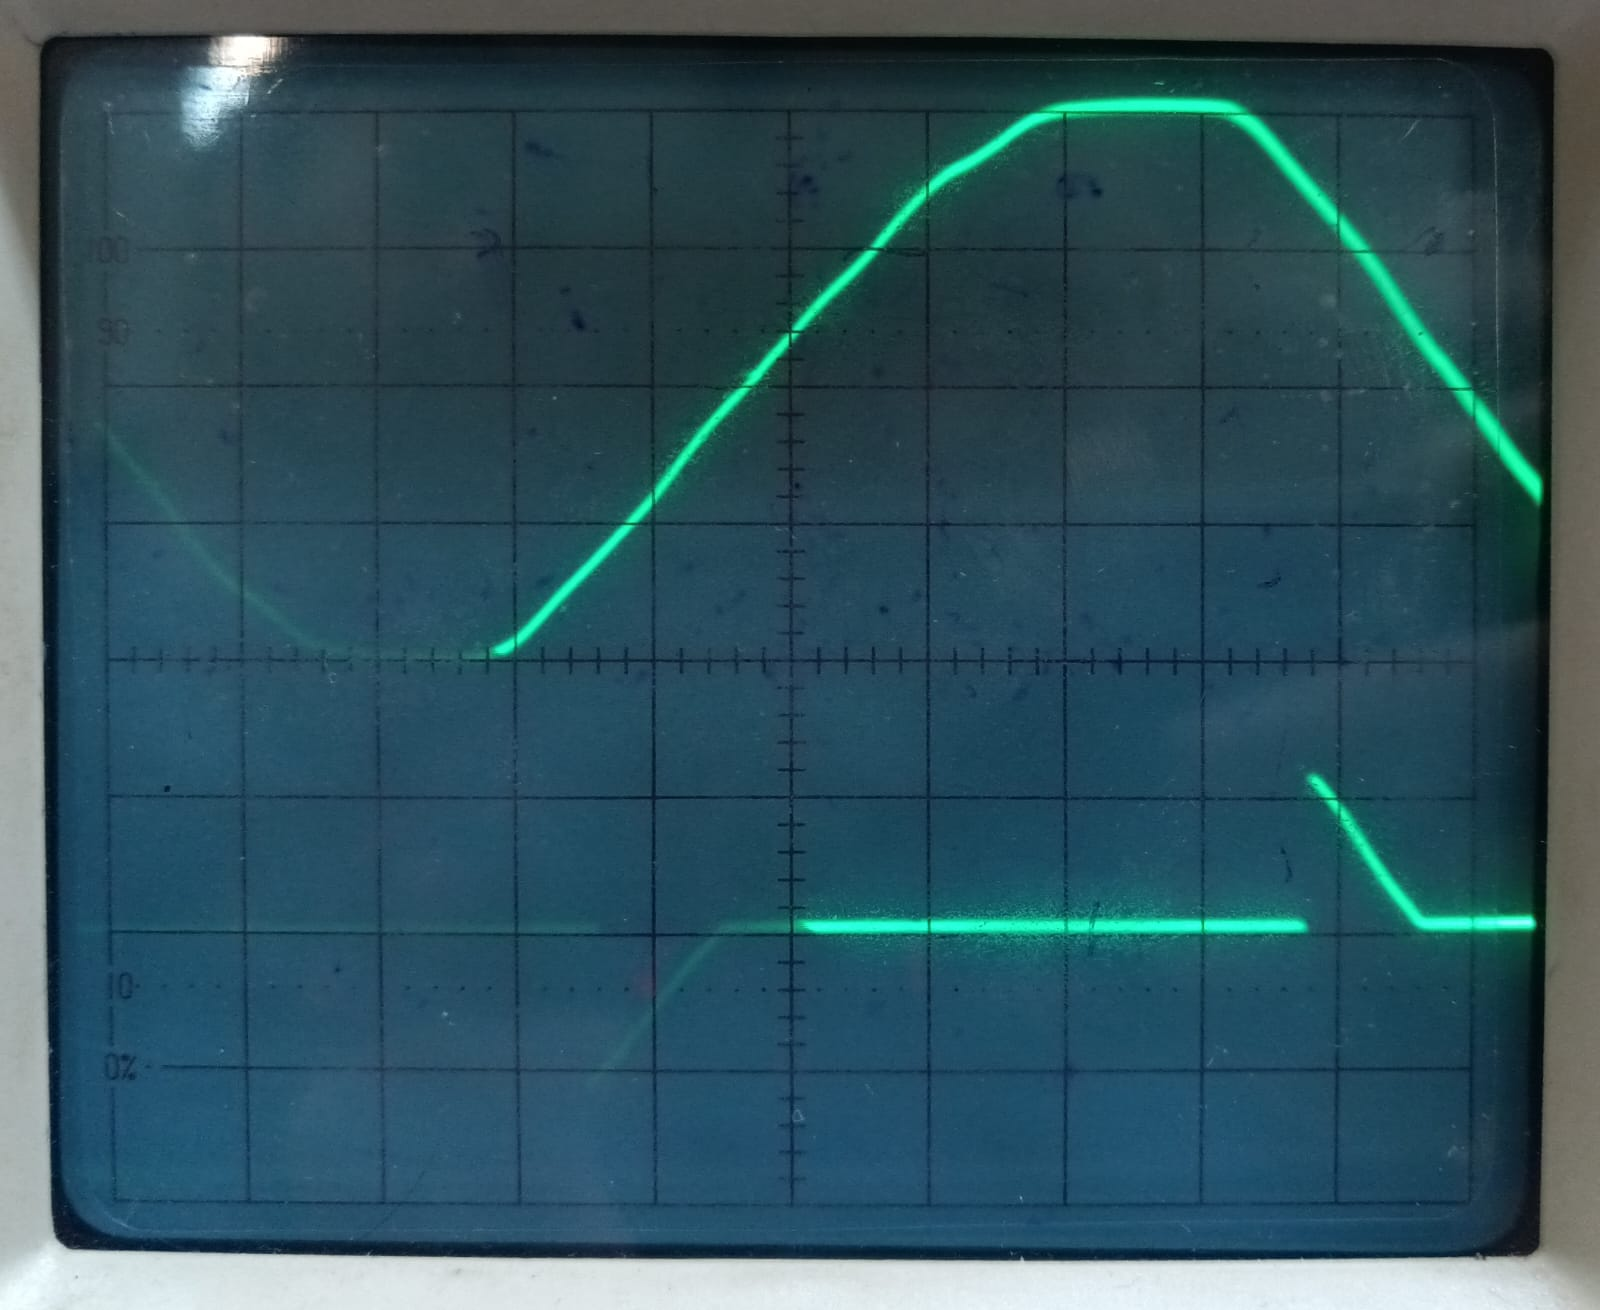
\includegraphics[width=0.65\textwidth]{Imagenes/30grad.jpeg}
        \label{}
        \caption{$Ang_{cond}=30$°}
    \end{subfigure}
    \hfill
        \begin{subfigure}[b]{0.5\textwidth}
        \centering  
            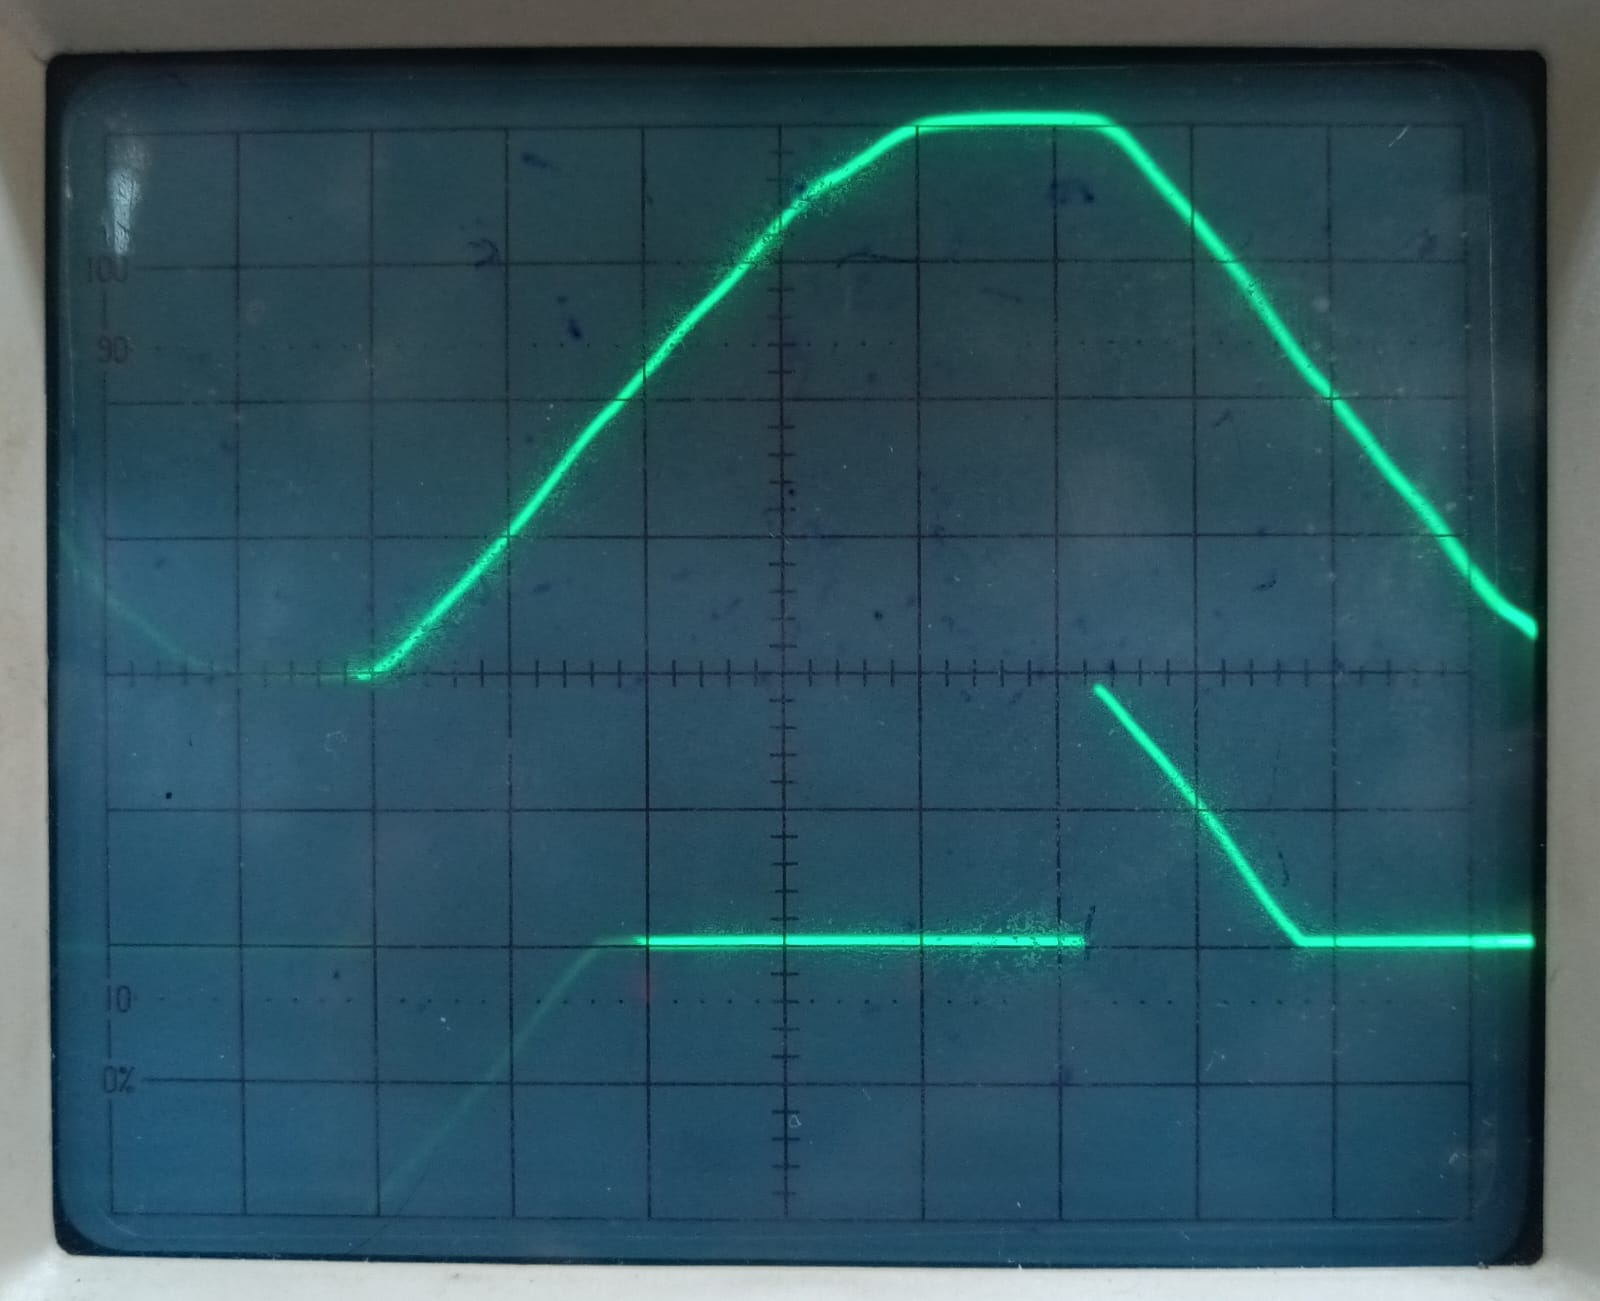
\includegraphics[width=0.65\textwidth]{Imagenes/60grad.jpeg}
        \label{}
        \caption{$Ang_{cond}=60$°}
    \end{subfigure}
    \hfill
        \begin{subfigure}[b]{0.49\textwidth}
        \centering  
            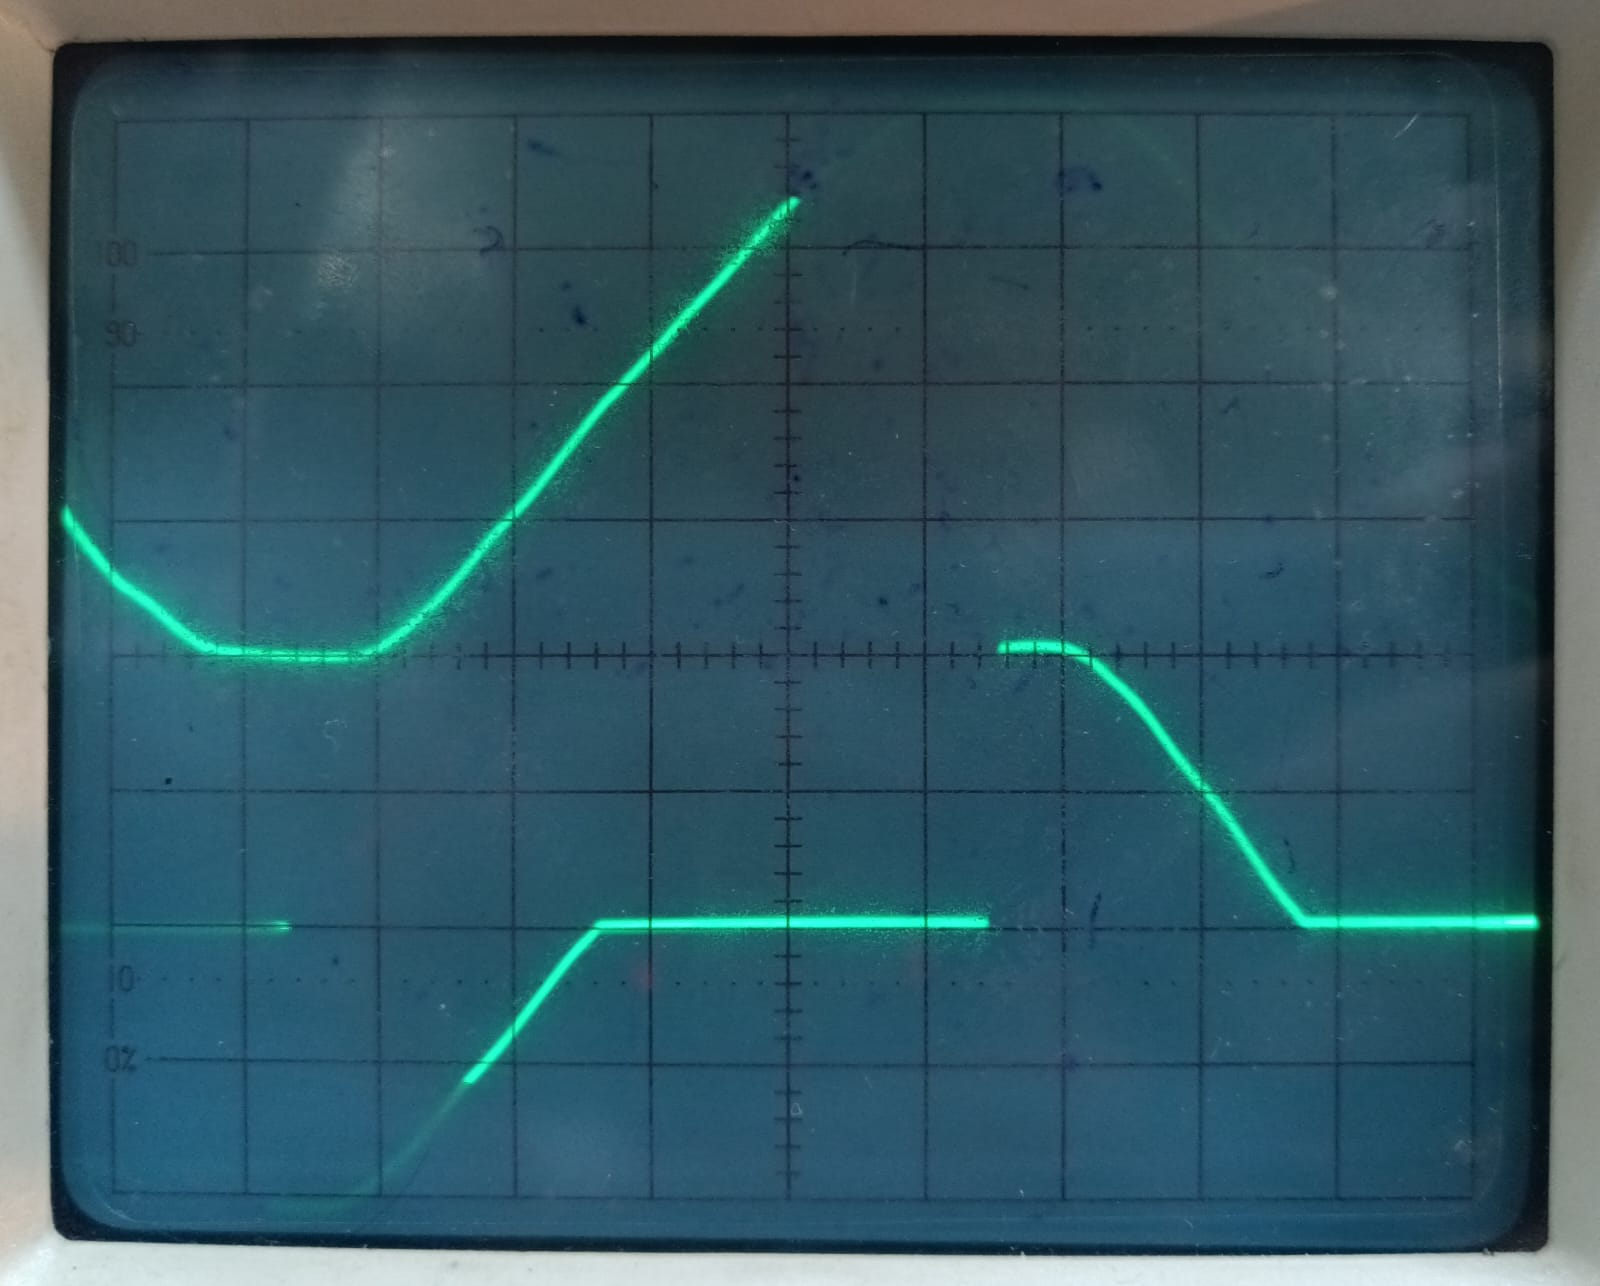
\includegraphics[width=0.65\textwidth]{Imagenes/90grad.jpeg}
        \label{}
        \caption{$Ang_{cond}=90$°}
    \end{subfigure}
    \hfill
        \begin{subfigure}[b]{0.5\textwidth}
        \centering  
            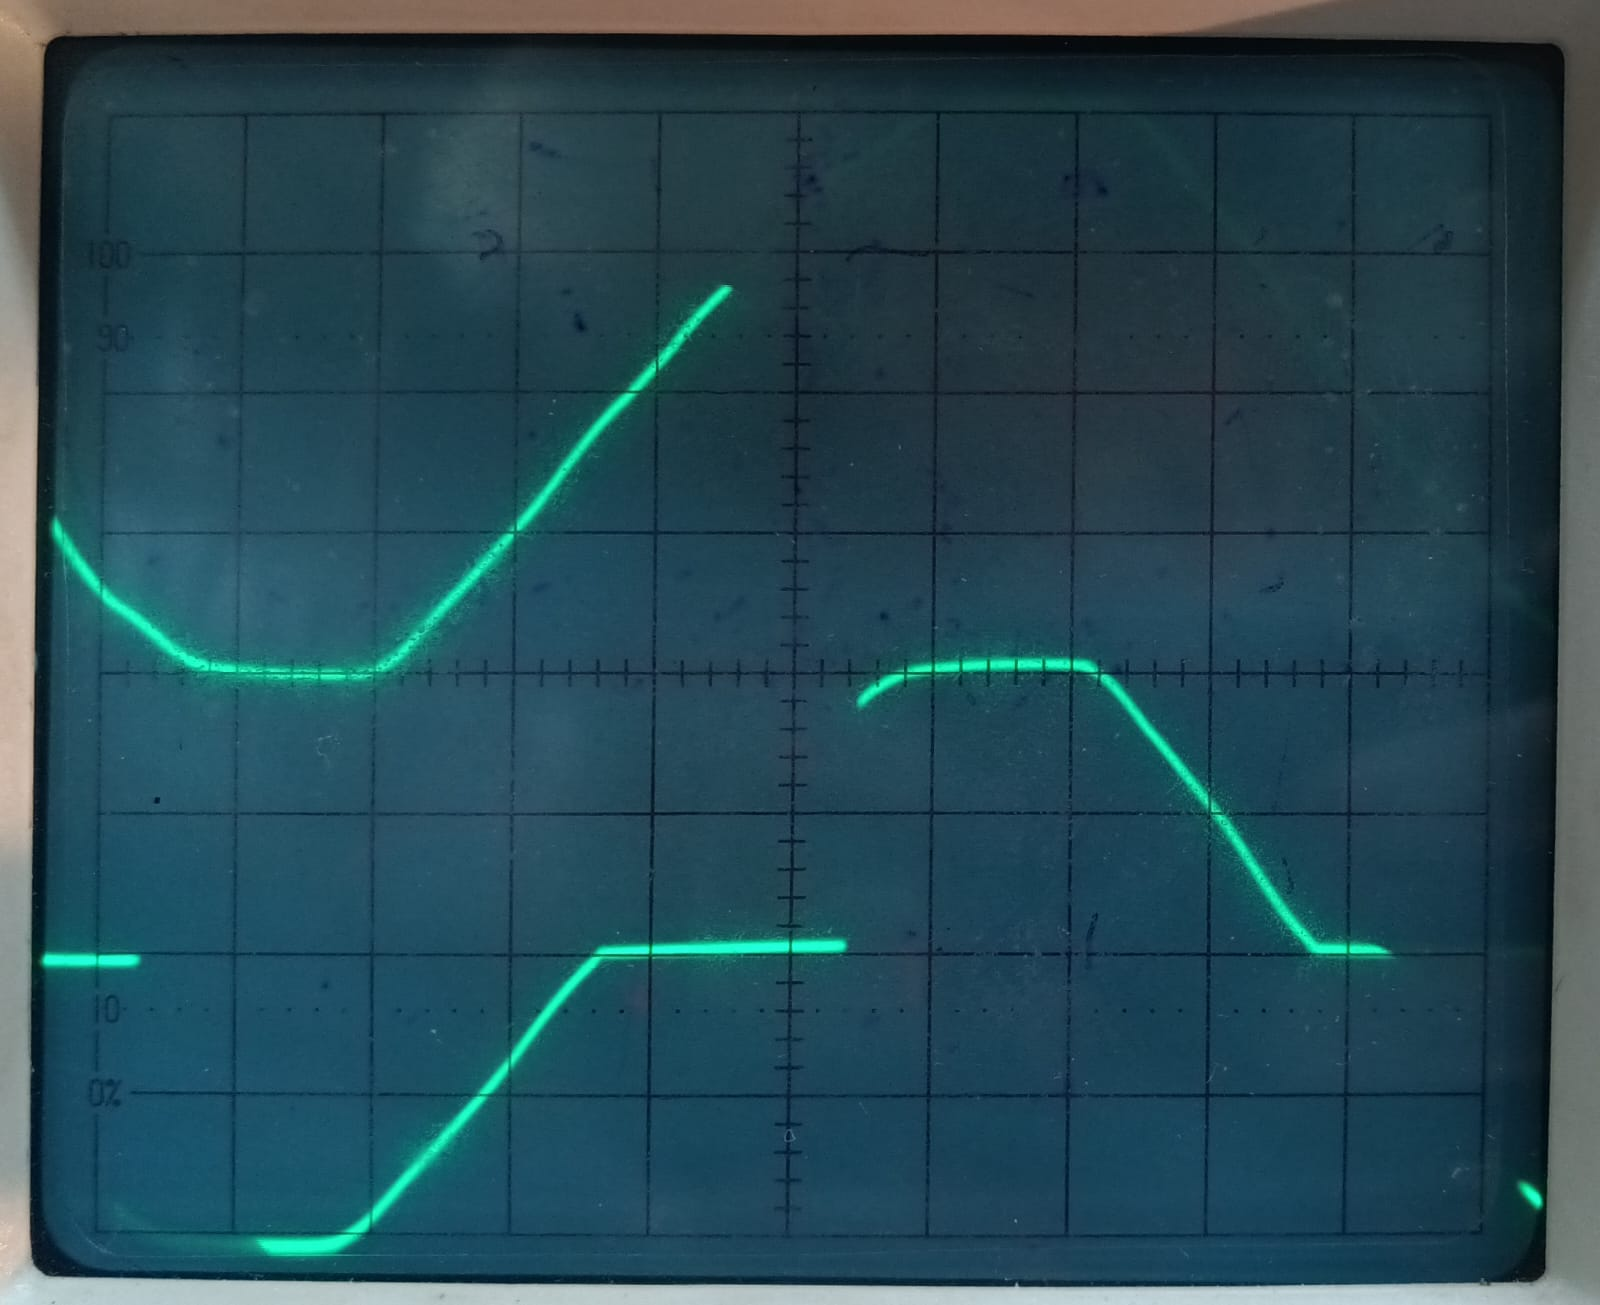
\includegraphics[width=0.65\textwidth]{Imagenes/120grad.jpeg}
        \label{}
        \caption{$Ang_{cond}=120$°}
    \end{subfigure}
    \hfill
        \begin{subfigure}[b]{0.49\textwidth}
        \centering  
            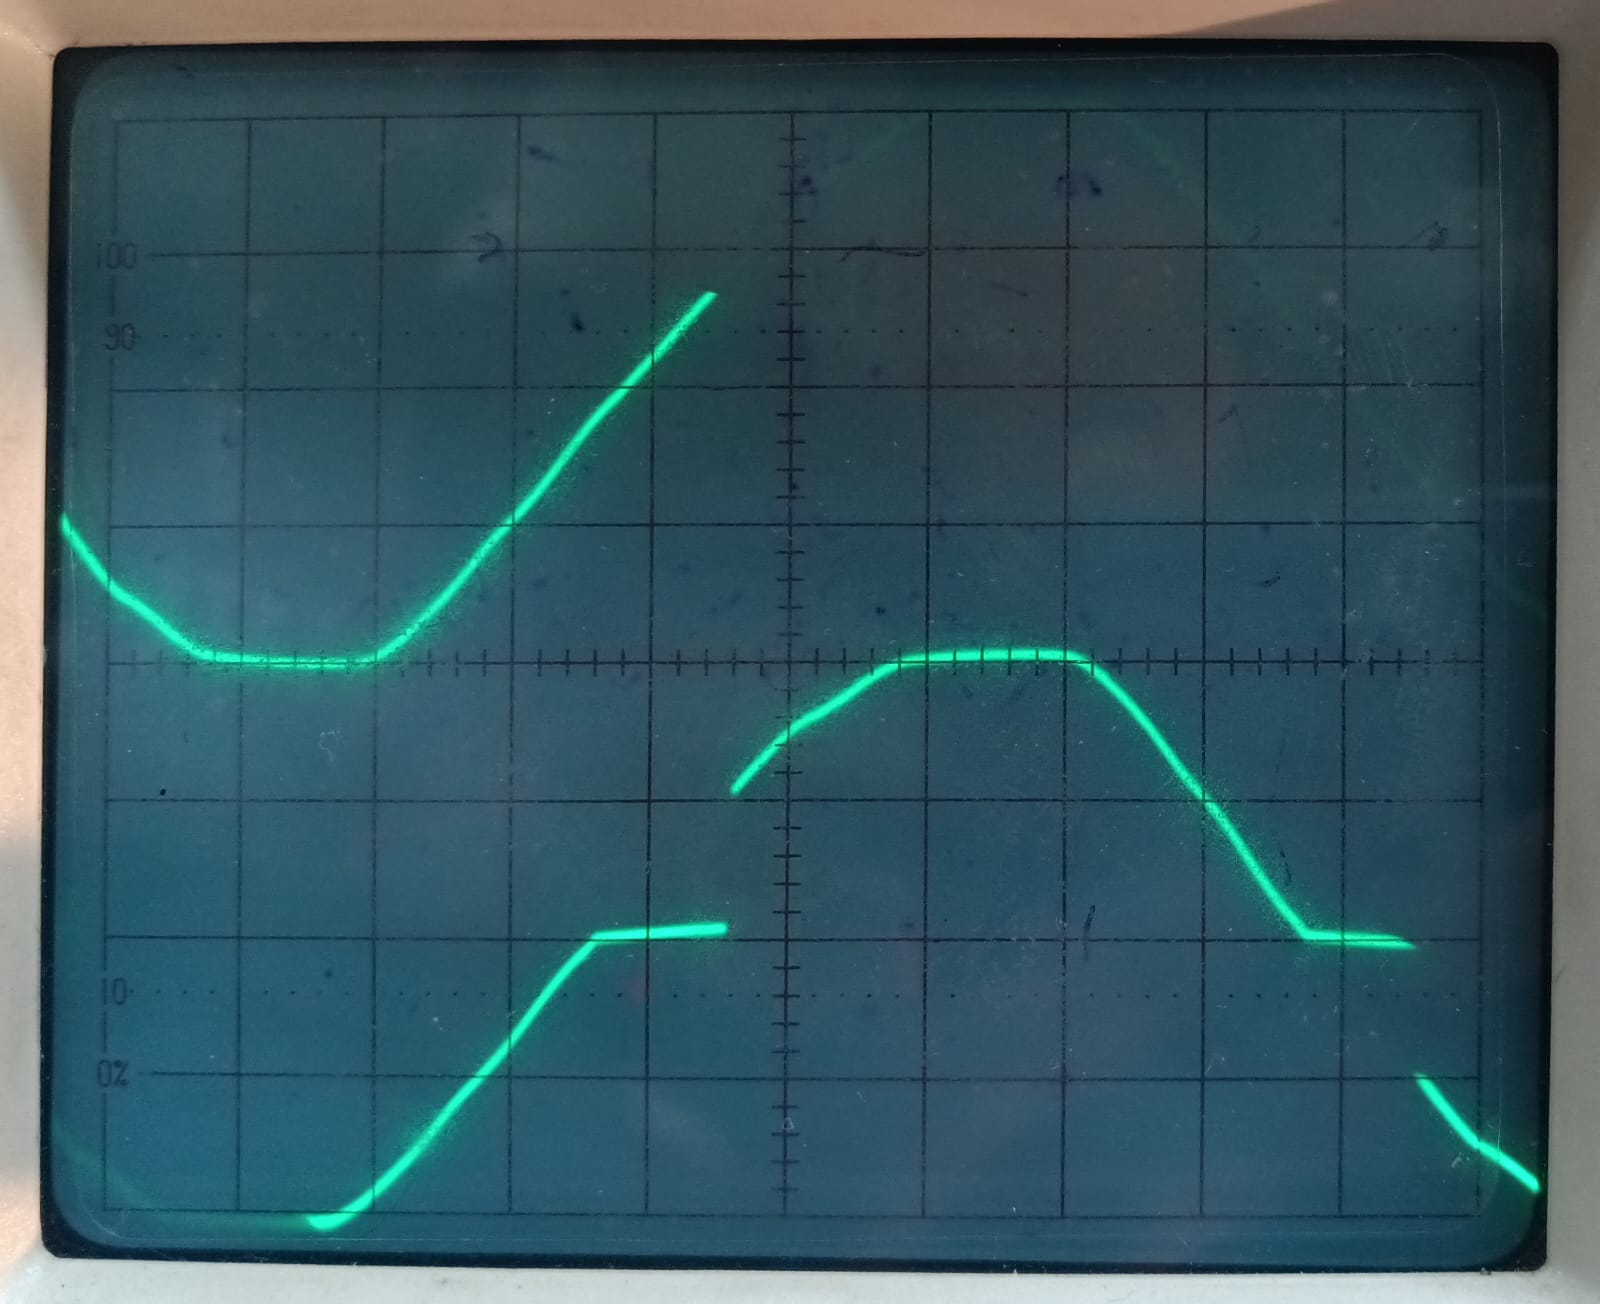
\includegraphics[width=0.65\textwidth]{Imagenes/150grad.jpeg}
        \label{}
        \caption{$Ang_{cond}=150$°}
    \end{subfigure}
    \caption{Señales con diferentes ángulos de conducción}
    \label{fig:fot_exp4}
    \end{center}
\end{figure}



Se pudo observar que el valor medido por el multimetro de respuesta al valor medio se aproxima al medido por el multimetro \textit{TrueRMS} a medida que la señal $V_o$ se aproxima a una señal sinusoidal. 

\unsubsubsection{Gráficos}

\begin{figure}[H]
    \centering
    \begin{tikzpicture}[scale=1]
        \coordinate (a1) at (0,0);
        \coordinate (a2) at (2,0.186*4);
        \coordinate (a3) at (4,0.386*4);
        \coordinate (a4) at (6,0.503*4);
        \coordinate (a5) at (8,0.906*4);
        \coordinate (a6) at (10,0.984*4);
        \coordinate (a7) at (12,1*4);

    \draw[thin,gray!40] (0,0) grid (12,4);
    \draw[<->] (0,0)--(12,0) node[right] {$[^\circ]$};
    \draw[<->] (0,0)--(0,4) node[above]{$\frac{V_o}{V_i}$};


    \foreach \a [evaluate={\y=int(\a*15)}] in {0,2,...,12}{
        \draw[line width=0.7pt,dotted] (\a,0) node[below]{\footnotesize $\y^\circ$};
    }
    \foreach \a [evaluate={\y=(\a*0.25)}] in {0,1,...,4}{
        \draw[line width=0.7pt,dotted] (0,\a) node[left]{\footnotesize $\y$};
    }
    \foreach \a in{1,...,7}{
       \draw[thin,dashed,black] let \p1=(a\a) in (\x1,0)--(a\a);
       \draw[line width=1pt,black](a\a) circle(1pt);
    }
    \foreach \x [evaluate={\y=int(\x+1);}] in {1,...,6}{
        \draw[line width=1pt,black] (a\x) -- (a\y);
   }
    
\end{tikzpicture}
\caption*{$V_o$ medido por el multimetro \textit{TrueRMS}}
    \begin{tikzpicture}[scale=1]
        \coordinate (a1) at (0,0);
        \coordinate (a2) at (2,0.074*4);
        \coordinate (a3) at (4,0.204*4);
        \coordinate (a4) at (6,0.295*4);
        \coordinate (a5) at (8,0.767*4);
        \coordinate (a6) at (10,0.931*4);
        \coordinate (a7) at (12,1*4);

    \draw[thin,gray!40] (0,0) grid (12,4);
    \draw[<->] (0,0)--(12,0) node[right] {$[^\circ]$};
    \draw[<->] (0,0)--(0,4) node[above]{$\frac{V_o}{V_i}$};


    \foreach \a [evaluate={\y=int(\a*15)}] in {0,2,...,12}{
        \draw[line width=0.7pt,dotted] (\a,0) node[below]{\footnotesize $\y^\circ$};
    }
    \foreach \a [evaluate={\y=(\a*0.25)}] in {0,1,...,4}{
        \draw[line width=0.7pt,dotted] (0,\a) node[left]{\footnotesize $\y$};
    }
    \foreach \a in{1,...,7}{
       \draw[thin,dashed,black] let \p1=(a\a) in (\x1,0)--(a\a);
       \draw[line width=1pt,black](a\a) circle(1pt);
    }
    \foreach \x [evaluate={\y=int(\x+1);}] in {1,...,6}{
        \draw[line width=1pt,black] (a\x) -- (a\y);
   }
    
\end{tikzpicture}
\caption*{$V_o$ medido por el multimetro con respuesta $V_{media}$}
   % \begin{tikzpicture}[scale=1]
\def\scal{1.5}
        \coordinate (a1) at (0,0);
        \coordinate (a2) at (2,1.52*\scal);
        \coordinate (a3) at (4,0.89*\scal);
        \coordinate (a4) at (6,0.7*\scal);
        \coordinate (a5) at (8,0.18*\scal);
        \coordinate (a6) at (10,0.05*\scal);
        \coordinate (a7) at (12,0);

    \draw[thin,gray!40,ystep=\scal] (0,0) grid (12,4);
    \draw[<->] (0,0)--(12,0) node[right] {$[^\circ]$};
    \draw[<->] (0,0)--(0,4) node[above]{$\kappa$};


    \foreach \a [evaluate={\y=int(\a*15)}] in {0,2,...,12}{
        \draw[line width=0.7pt,dotted] (\a,0) node[below]{\footnotesize $\y^\circ$};
    }
    \foreach \a [evaluate={\y=int(\a+1)}] in {0,1,...,2}{
        \draw[line width=0.7pt,dotted] (0,\a*\scal) node[left]{\footnotesize $\y$};
    }
    \foreach \a in{1,...,7}{
       \draw[thin,dashed,black] let \p1=(a\a) in (\x1,0)--(a\a);
       \draw[line width=1pt,black](a\a) circle(1pt);
    }
    \foreach \x [evaluate={\y=int(\x+1);}] in {1,...,6}{
        \draw[line width=1pt,black] (a\x) -- (a\y);
   }
    
\end{tikzpicture}
\caption*{Factor de corrección $\kappa=\frac{V_{TRms}}{V_{MRms}}$ }
    \label{fig:vivo}
\end{figure}

\unsubsubsection{Factor de Corrección}

\begin{figure}[H]
    \centering
    \begin{tikzpicture}[scale=1]
\def\scal{1.5}
        \coordinate (a1) at (0,0);
        \coordinate (a2) at (2,1.52*\scal);
        \coordinate (a3) at (4,0.89*\scal);
        \coordinate (a4) at (6,0.7*\scal);
        \coordinate (a5) at (8,0.18*\scal);
        \coordinate (a6) at (10,0.05*\scal);
        \coordinate (a7) at (12,0);

    \draw[thin,gray!40,ystep=\scal] (0,0) grid (12,4);
    \draw[<->] (0,0)--(12,0) node[right] {$[^\circ]$};
    \draw[<->] (0,0)--(0,4) node[above]{$\kappa$};


    \foreach \a [evaluate={\y=int(\a*15)}] in {0,2,...,12}{
        \draw[line width=0.7pt,dotted] (\a,0) node[below]{\footnotesize $\y^\circ$};
    }
    \foreach \a [evaluate={\y=int(\a+1)}] in {0,1,...,2}{
        \draw[line width=0.7pt,dotted] (0,\a*\scal) node[left]{\footnotesize $\y$};
    }
    \foreach \a in{1,...,7}{
       \draw[thin,dashed,black] let \p1=(a\a) in (\x1,0)--(a\a);
       \draw[line width=1pt,black](a\a) circle(1pt);
    }
    \foreach \x [evaluate={\y=int(\x+1);}] in {1,...,6}{
        \draw[line width=1pt,black] (a\x) -- (a\y);
   }
    
\end{tikzpicture}
\caption*{Factor de corrección $\kappa=\frac{V_{TRms}}{V_{MRms}}$ }
\end{figure}



\newpage
\subsection{Experimento 5: Determinación de la Resistencia de salida a lazo abierto y a lazo cerrado}
Las mediciones fueron realizadas sobre un amplificador realimentado que se encontraba preparado en el Laboratorio de Electrónica, presentado en la sección \ref{sec:Amp2}. 

%Este amplificador cuenta con 4 resistencias a las salida de diferentes valores, las cuales se pueden seleccionar con un jumper para que sea nuestra carga. 

Para este experimento se realizó la siguiente conexión para comenzar con las mediciones.

\begin{figure}[H]
    \centering
    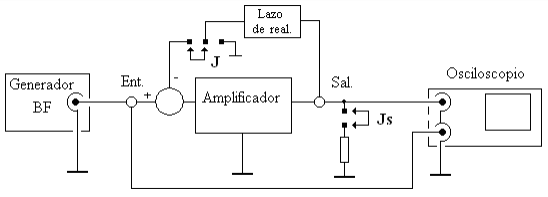
\includegraphics[width=0.9\textwidth]{Imagenes/conexion_p5.png}
    \caption{Esquema de medición}
    \label{fig:esq_conexion}
\end{figure}

En primer lugar se realizaron las mediciones a lazo abierto y sin carga, por lo tanto el jumper \textbf{J} se conecto entre 2 y 3; y el jumper \textbf{Js} se deja desconectado. En estas condiciones se configuró el generador de funciones para introducir en la entrada una señal sinusoidal de 1 kHz y  se ajusto el nivel, de manera que la forma de onda de salida tenga la máxima amplitud libre de distorsión por recorte.

Con el osciloscopio se midió la tensión de la señal de salida y de la señal de entrada (figura \ref{fig:amp2LA}), para así, obtener el valor de la ganancia a lazo abierto. 

\begin{figure}[H]
    \centering
    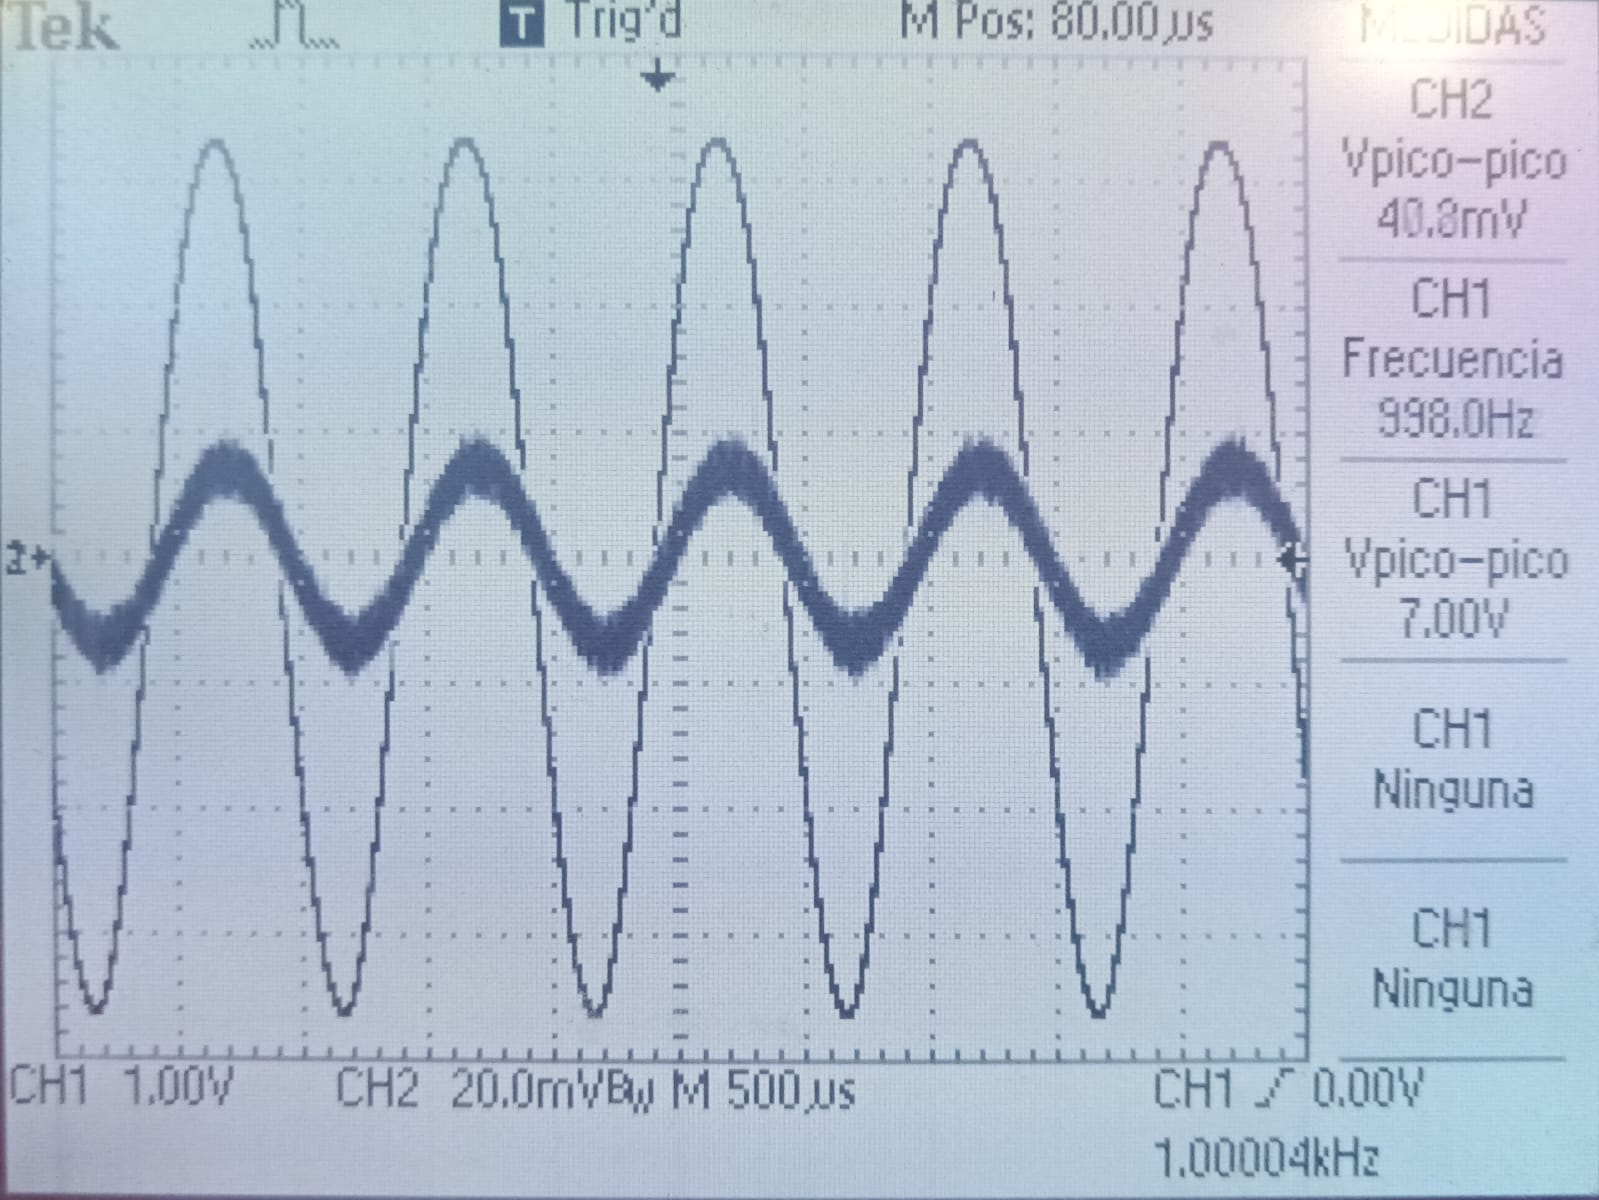
\includegraphics[width=0.6\textwidth]{Imagenes/Amp2LA.jpeg}
    \caption{Señal de entrada y salida, a lazo abierto}
    \label{fig:amp2LA}
\end{figure}

Los datos medidos y calculados se pueden apreciar en la tabla \ref{tab:exp5}.

\begin{table}[H]
    \centering
    \scalebox{1}{
    \begin{tabular}{|c|c|c|}
    \hline
         $V_i$ [$mV_{pp}$] & $V_o$ [$V_{pp}$] & $A=\cfrac{V_o}{V_i}$  [\ohm] \\
    \hline
        40  & 7  & 175\\
    \hline
        \end{tabular}}
        \def\tablename{Tabla} 
        \caption{Valores medidos de tensión y ganancia calculada}
        \label{tab:exp5}
\end{table}

Luego, se procedió a conectar la resistencia de 1 k\ohm ~como resistencia de carga mediante el jumper \textit{JS}, y se procedió a medir nuevamente la tensión de salida. 

Con estos valores de tensión en vacío y con una carga conectada, es posible mediante un cálculo, obtener el valor de resistencia de salida \textit{Ro} del amplificador. A continuación, se presentan los datos en la tabla \ref{tab1:exp5b}.

\begin{table}[H]
    \centering
    \scalebox{1}{
    \begin{tabular}{|c|c|c|}
    \hline
         $V_o$ [$V_{pp}$] & $V_s$ [$V_{pp}$] & $R_o= R_l \cdot (\cfrac{V_o}{V_s}-1)$ [\ohm]\\
    \hline
        7  & 4,52 & 548,67 \\
    \hline
        \end{tabular}}
        \def\tablename{Tabla} 
        \caption{Valores de tensión medidos y resistencia calculada}
        \label{tab1:exp5b}
\end{table}


Una vez obtenido las mediciones a lazo abierto, se conectó el jumper \textit{J} entre 1 y 2, cerrando el lazo, y se realizaron nuevamente los mismos pasos que anteriormente, se desconectó la carga y se configuró la amplitud del generador para obtener la máxima tensión de entrada que no recorte la señal de salida. Una vez todo configurado se volvieron a efectuar las mediciones (figura \ref{fig:amp2LC}) pero ahora, en condición de realimentación (tabla \ref{tab:exp5c}). 

\begin{figure}[H]
    \centering
    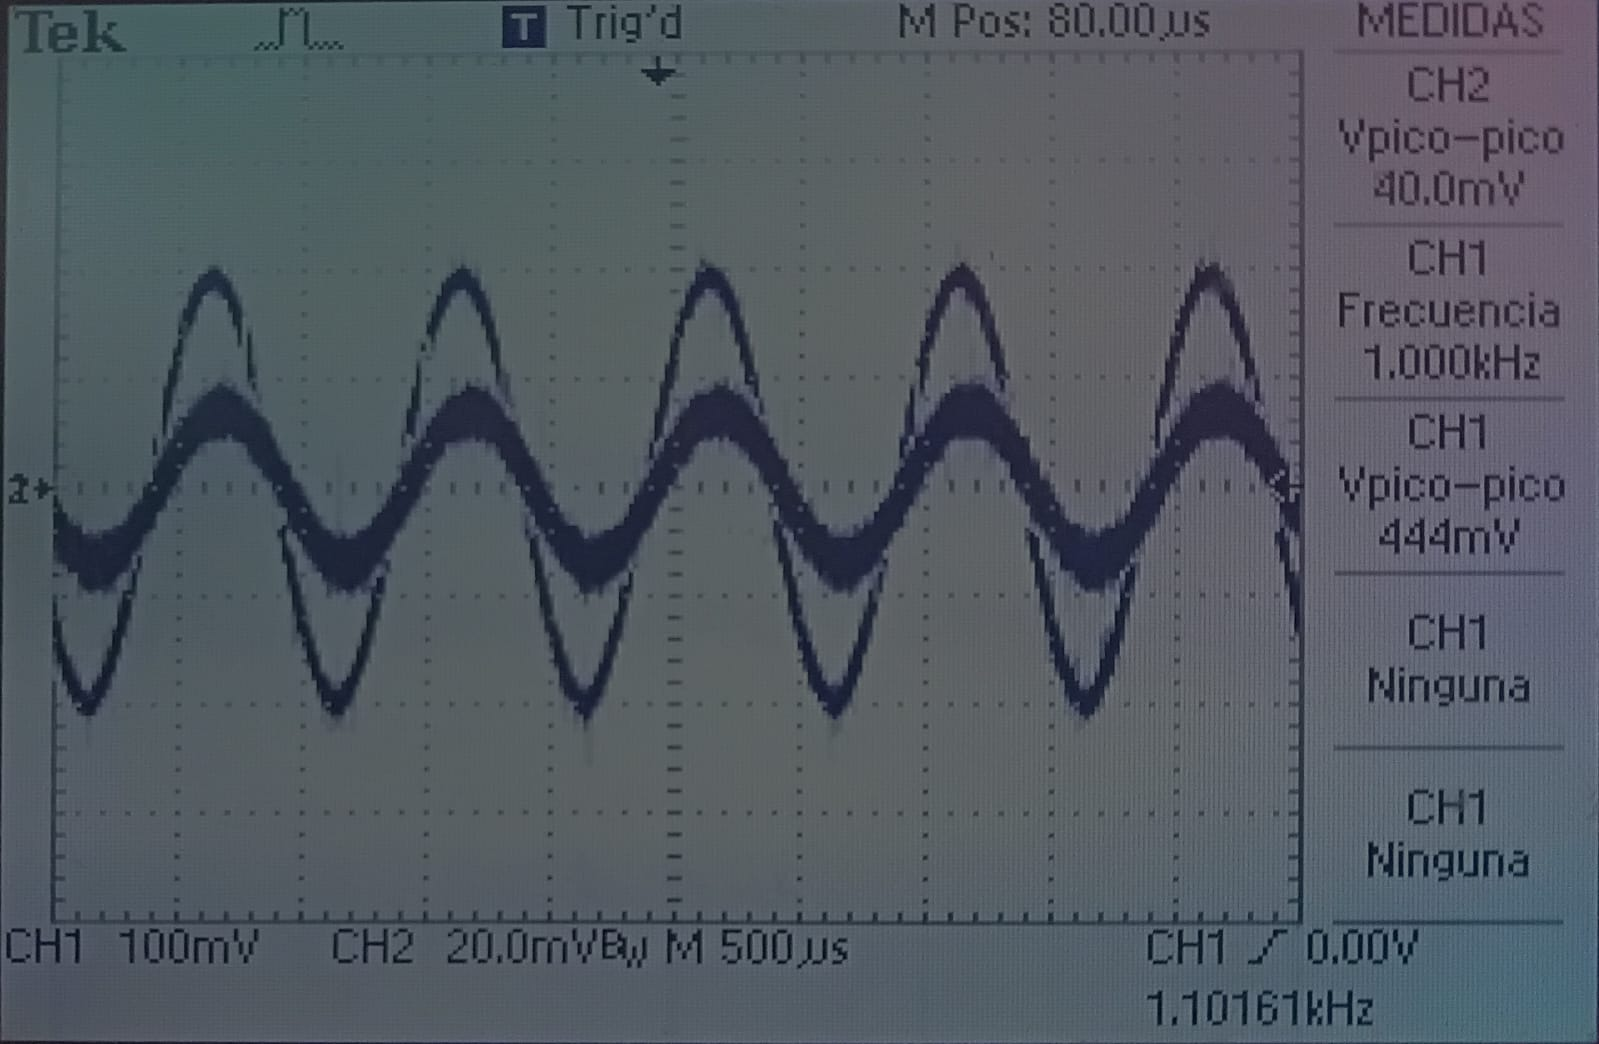
\includegraphics[width=0.6\textwidth]{Imagenes/Amp2LC.jpeg}
    \caption{Señal de entrada y salida, a lazo cerrado}
    \label{fig:amp2LC}
\end{figure}


\begin{table}[H]
    \centering
    \scalebox{1}{
    \begin{tabular}{|c|c|c|}
    \hline
         $V_i$ [$mV_{pp}$] & $V_o$'[$mV_{pp}$] & $G=\cfrac{V_o'}{V_i}$ \\
    \hline
        40  & 444 & 11,1\\
    \hline
        \end{tabular}}
        \def\tablename{Tabla} 
        \caption{Valores medidos de tensión y ganancia calculada}
        \label{tab:exp5c}
\end{table}

Con los valores de tensión de entrada y salida y la ganancia a lazo cerrado ya es posible obtener el valor de resistencia de salida del circuito con realimentación \textbf{$R_0'$} utilizando la siguiente fórmula (ecuación \ref{eq:Rop}):

\begin{equation}
     R_0'= \frac{R_o \cdot G}{A}= \cfrac{548,67 [\ohm] \cdot 11,1}{175}= 34,8~\ohm
     \label{eq:Rop}
\end{equation}

Otra forma de  obtener la Resistencia de salida a lazo cerrado \textbf{Ro'}, es midiendo la tensión de salida con una carga conectada, esta resistencia debe ser de un valor bajo. En el amplificador en cuestión hay dos valores que se pueden usar, una de 100\ohm y una de 33\ohm. 

Para comprobar cuánta variación producía el usar una u otra resistencia, de realizaron las mediciones con las dos resistencias obteniendo los siguientes valores:

\vspace{0.5cm}
\textbf{Con $R_l$= 100~\ohm}:

\begin{table}[H]
    \centering
    \scalebox{1}{
    \begin{tabular}{|c|c|c|}
    \hline
         $V_o$ [$mV_{pp}$] & $V_s$ [$mV_{pp}]$ & $R_o' = R_l \cdot (\cfrac{V_o}{V_s}-1)$ [\ohm]\\
    \hline
        444  & 300 & 48 \\
    \hline
        \end{tabular}}
        \def\tablename{Tabla} 
        \caption{Valores de tensión medidos y resistencia calculada}
        \label{tab:exp5d}
\end{table}

\textbf{Con $R_l$= 33~\ohm}:

\begin{table}[H]
    \centering
    \scalebox{1}{
    \begin{tabular}{|c|c|c|}
    \hline
         $V_o$ [$mV_{pp}$] & $V_s$ [$mV_{pp}]$ & $R_o'= R_l \cdot (\cfrac{V_o}{V_s}-1)$ [\ohm]\\
    \hline
         444 & 204 & 38.824 \\
    \hline
        \end{tabular}}
        \def\tablename{Tabla} 
        \caption{Valores de tensión medidos y resistencia calculada}
        \label{tab:exp5e}
\end{table}

Como era de esperarse, estos dos últimos resultados no coincidieron con el valor calculado de la resistencia de salida a lazo cerrado, y esto fue así debido a la misma naturaleza del circuito, que intenta mantener la ganancia estable, haciendo que la tensión de salida no se modifique y para esto, el amplificador modificará su impedancia de salida interna.

%\newpage
\vspace{1.5cm}
\subsection{Experimento 6: Medición de la potencia eficaz máxima de salida}

Mediante este ensayo, se pretende calcular el valor de la potencia eficaz máxima de salida del amplificador, tanto a lazo abierto, como cerrado. Para llegar a esto, se medirá la tensión de salida máxima del amplificador (sin distorciones), con una resistencia de carga igual a la impedancia de salida obtenida en la sección anterior ($R_o$, para lazo abierto y $R_o'$, para lazo cerrado) y en base a eso, mediante una fórmula se calculará la potencia máxima de salida. 

Los fundamentos de este experimento se encuentran en la sub-sección \ref{sec:MaxPot}, del Marco Teórico.

%\subsubsection{Fundamento}

\subsubsection{Implementación y Mediciones}

Se empleará el mismo circuito amplificador que en el experimento anterior (\ref{fig:esq_amp_tp3}), pero conectado de la siguiente manera (figura \ref{fig:circ6}):

\begin{figure}[H]
    \centering
    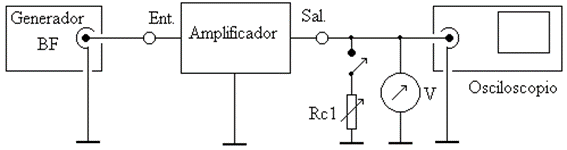
\includegraphics[width=0.85\textwidth]{Imagenes/circ6.png}
    \caption{Diagrama del circuito a ensayar}
    \label{fig:circ6}
\end{figure}

Como se explicó, la resistencia de carga $R_{C1}$ deberá ser igual a $R_o$ para lazo abierto. Revisando el circuito en la figura \ref{fig:esq2_amp_tp3}, se ve que colocando un jumper en la posición \textit{JS4}, se coloca como resistencia de carga una resistencia de 560 $\Omega$, muy similar a $R_o$. 

Una vez allí, se configura la frecuencia del generador a 1 kHz y se varía la amplitud hasta obtener la máxima salida antes de que recorte. En este caso el valor de tensión obtenido fue de 4,2 $V_{pp}$. 

Ahora se repetirá el mismo procedimiento pero para el amplificador realimentado (lazo cerrado), y cambiando el jumper de a la posición \textit{JS1}, haciendo que ahora la resistencia de carga $R_{C1}$ sea de 33 $\Omega$, un valor bastante próximo al de $R_o'$. En este caso, la tensión máxima de salida fue de 508 $mV_{pp}$.


\subsubsection{Cálculos}

Finalmente para calcular la potencia máxima de transferencia de nuestro amplificador, se empleará la siguiente fórmula (ecuación \ref{eq:potmax}):

\begin{equation}
    P_{max} = \cfrac{V_{rms}^2}{R} = \cfrac{V_{pp}^2}{8R}
    \label{eq:potmax}
\end{equation}

Obteniendo los siguientes valores como resultado (tabla \ref{tab:exp6}):

\begin{table}[H]
    \centering
    \scalebox{1}{
    \begin{tabular}{|c|c|c|}
    \hline
          & Lazo abierto & Lazo cerrado \\
          & ($R_{C1}=R_o$) & ($R_{C1}=R_o'$) \\
    \hline
        P [mW]  & 3.938 & 0.978 \\
    \hline
        \end{tabular}}
        \def\tablename{Tabla} 
        \caption{Potencias calculadas}
        \label{tab:exp6}
\end{table}


\newpage
\subsection{Experimento 7: Ensayo de la respuesta en frecuencia (ancho de banda) del amplificador}
Esta parte del trabajo practico, tiene como objetivo graficar y determinar la respuesta en frecuencia del amplificador, además de medir su ancho de banda. Los puntos de mayor interés serán las curvas de subida y bajada de ganancia que, generalmente, son marcadas por un cambio de tendencia cuando la respuesta del amplificador es de $-3\mathrm{dB}$ en comparación de su ganancia máxima en máxima excursión simétrica. Las frecuencias que generan una respuesta de $-3\mathrm{dB}$ se nombran como frecuencias de corte. La diferencia entre las frecuencias de corte da como resultado el ancho de banda del amplificador.

Teniendo en cuenta esto se ajusto la señal de entrada al amplificador, tanto a lazo abierto como a lazo cerrado, para obtener la señal de salida en máxima excursión simétrica. Luego matemáticamente se obtuvieron los valores de tensión esperados en la salida para las frecuencias de corte.

Se determino que en nivel de tensión ($V_{pp}$) de la señal de salida a lazo abierto sin saturación es de $V_{ppS}=7V$.Esta señal de salida le corresponde a una señal de entrada de $V_{ppE}=170mV$.
Teniendo en cuenta la ecuación para determinar la ganancia en $dB$ de tensión \ref{eq:dBaveces}, se calculo el nivel esperado de tensión ($V_{out}$) para las frecuencias de corte a lazo abierto:
\begin{equation}
    V_{out}=7V\cdot10^{\frac{-3}{20}}\lrah V_{out}=4,95V
\end{equation}

Se realizo el barrido de frecuencia y se determinaron las frecuencias de corte.
\begin{table}[H]
\parbox{.45\textwidth}{  
    \centering
    \begin{tabular}{|c|c|c|}
        \hline
        $f$ [Hz] &  $V_{pp}$&$GR_{dB}$\\
        \hline
         $750$&$6,92$&$-0.10$\\ 
         $500$&$6,76$&$-0.30$\\ 
         $250$&$6,52$&$-0.62$\\ 
         $150$&$6,28$&$-0.94$\\ 
         $100$&$6,00$&$-1.34$\\ 
         $75$&$5,56$&$-2.00$\\
         $65$&$5,32$&$-2.38$\\
         $54$&$4,96$&$-2.99$\\
         \hline
    \end{tabular}
    \caption{Barrido descendente}
    \label{tab:RF-LAAinf}
    }
    \parbox{.45\textwidth}{
    \centering
    \begin{tabular}{|c|c|c|}
        \hline
        $f$ [kHz] &  $V_{pp}$&$GR_{dB}$\\
        \hline
         $10$&$7,00$&$-0.00$\\ 
         $30$&$6,90$&$-0.12$\\ 
         $50$&$6,28$&$-0.94$\\ 
         $60$&$5,88$&$-1.51$\\ 
         $70$&$5,56$&$-2.00$\\
         $75$&$5,36$&$-2.32$\\
         $78$&$5,28$&$-2.45$\\
         $80$&$5,24$&$-2.51$\\
         $85$&$5,00$&$-2.92$\\
         $87$&$4,96$&$-2.99$\\
         \hline
    \end{tabular}
    \caption{Barrido ascendente}
    \label{tab:RF-LAAsup}
    }
\end{table}
Como se observa en las tablas \ref{tab:RF-LAAinf} y \ref{tab:RF-LAAsup}, la frecuencia de corte correspondiente a la curva de subida de ganancia es de $F_{CAinf}=54_{Hz}$ y la frecuencia de corte correspondiente a la curva de bajada de ganancia es de $F_{CAsup}=87_{kHz}$. Dando como resultado un ancho de banda de:
\begin{equation*}
    AB_{LA} = F_{CAsup}-F_{CAinf}\lrah AB_{LA}=86.946 kHz
\end{equation*}

\begin{figure}[H]
    \centering
    \begin{tikzpicture}[scale=1]

    \def\scalya{3}
    \def\scaly{1}
    \def\scalxa{3}
    \def\scalx{2}
    
    %datosLineaA
    \coordinate (a8) at ({log10(750)*\scalx},{20*log10(6.92/7)*\scaly+\scalya});
    \coordinate (a7) at ({log10(500)*\scalx},{20*log10(6.76/7)*\scaly+\scalya});
    \coordinate (a6) at ({log10(250)*\scalx},{20*log10(6.52/7)*\scaly+\scalya});
    \coordinate (a5) at ({log10(150)*\scalx},{20*log10(6.28/7)*\scaly+\scalya});
    \coordinate (a4) at ({log10(100)*\scalx},{20*log10(6.00/7)*\scaly+\scalya});
    \coordinate (a3) at ({log10(75)*\scalx},{20*log10(5.56/7)*\scaly+\scalya});
    \coordinate (a2) at ({log10(65)*\scalx},{20*log10(5.32/7)*\scaly+\scalya});
    \coordinate (a1) at ({log10(54)*\scalx},{20*log10(4.96/7)*\scaly+\scalya});
    \coordinate (a9) at ({(log10(10)+\scalxa)*\scalx},{20*log10(7.00/7)*\scaly+\scalya});
    \coordinate (a10) at ({(log10(30)+\scalxa)*\scalx},{20*log10(6.90/7)*\scaly+\scalya});
    \coordinate (a11) at ({(log10(50)+\scalxa)*\scalx},{20*log10(6.28/7)*\scaly+\scalya});
    \coordinate (a12) at ({(log10(60)+\scalxa)*\scalx},{20*log10(5.88/7)*\scaly+\scalya});
    \coordinate (a13) at ({(log10(70)+\scalxa)*\scalx},{20*log10(5.56/7)*\scaly+\scalya});
    \coordinate (a14) at ({(log10(75)+\scalxa)*\scalx},{20*log10(5.36/7)*\scaly+\scalya});
    \coordinate (a15) at ({(log10(78)+\scalxa)*\scalx},{20*log10(5.28/7)*\scaly+\scalya});
    \coordinate (a16) at ({(log10(80)+\scalxa)*\scalx},{20*log10(5.24/7)*\scaly+\scalya});
    \coordinate (a17) at ({(log10(85)+\scalxa)*\scalx},{20*log10(5.00/7)*\scaly+\scalya});
    \coordinate (a18) at ({(log10(87)+\scalxa)*\scalx},{20*log10(4.96/7)*\scaly+\scalya});



    
    %Ejex
    \foreach \x [evaluate={\a=int(\x+1)}]in {0,...,5}{
    \foreach \y in {1,...,10}
        \draw[line width=1pt,gray!40] ({(\x+log10(\y))*\scalx},0)--({(\x+log10(\y))*\scalx},4);
        \draw[shift={(\a*\scalx,0)}] (0pt,2pt) -- (0pt,-2pt) node[below] {\footnotesize $10^\a$};
    }
    \draw[shift={(0,0)}] (0pt,2pt) -- (0pt,-2pt) node[below] {\footnotesize $10^0$};
    \draw[->] (0,0)--(12,0) node[right] {$Frec_{(Hz)}$};
    
    %Ejey
    \foreach \y [evaluate={\a=int(\y-3)}] in {1,...,4}{
        \draw[line width=1pt,gray!40] (0,\y)--(12,\y);
        \draw[shift={(0,\y)}] (2pt,0pt) -- (-2pt,0pt) node [left] {\footnotesize $\a$};
    }
   \draw[shift={(0,0)}] (2pt,0pt) -- (-2pt,0pt) node [left] {\footnotesize $-3$};
   \draw[<->] (0,0)--(0,4) node[left=8pt]{$GR_{dB}$};
   
   
    %Linea A
    \foreach \x  in {1,...,18}{
        \draw[line width=1.5pt,fill=black] (a\x) circle(1.5pt);
   }
   \foreach \x [evaluate={\y=int(\x+1);}] in {1,...,17}{
        \draw[line width=1pt,black] (a\x) -- (a\y);
   }
   
\end{tikzpicture}
    \caption{Respuesta en frecuencia de ganancia relativa a lazo abierto}
    \label{fig:RFA}
\end{figure}
Se repitió el mismo procedimiento para el caso de la configuración a lazo cerrado. Se observo que el valor máximo de tensión pico-pico a la salida en la configuración de lazo cerrado, que no genere distorsión, es de  $V_{ppS}=7.48$, correspondiente a una señal de tensión pico-pico a la entrada de $V_{ppE}=3.2$. Utilizando la ecuación \ref{eq:dBaveces} se obtuvo el nivel de tensión esperado a la salida para las frecuencias de corte:
\begin{equation}
    V_{out}=7.48V\cdot10^{\frac{-3}{20}}\lrah V_{out}=5,29V
\end{equation}
Se realizo el barrido de frecuencia obteniendo las siguientes tablas de datos.
\begin{table}[H]
\parbox{.45\textwidth}{  
    \centering
   \begin{tabular}{|c|c|c|}
        \hline
        $f$ [Hz] &  $V_{pp}$ & $GR_{dB}$\\
        \hline
         $500$&$7,48$&$0$\\ 
         $250$&$7,40$&$-0.09$\\ 
         $150$&$7,40$&$-0.09$\\ 
         $100$&$7,32$&$-0.19$\\ 
         $50$&$7,08$&$-0.48$\\
         $30$&$6,92$&$-0.67$\\
         $25$&$6,76$&$-0.88$\\
         $20$&$6,52$&$-1.19$\\
         $15$&$6,12$&$-1.74$\\
         $13$&$5,96$&$-1.97$\\
         $11$&$5,46$&$-2.73$\\
         $10$&$5,28$&$-3.02$\\
         \hline
    \end{tabular}
    \caption{Barrido descendente}
    \label{tab:RF-LACinf}
    }
    \parbox{.45\textwidth}{
    \centering
    \begin{tabular}{|c|c|c|}
        \hline
        $f$ [kHz] &  $V_{pp}$&$GR_{dB}$\\
        \hline
         $30$&$7,48$&$0$\\ 
         $50$&$7,50$&$0.05$\\ 
         $100$&$7,46$&$0.05$\\ 
         $150$&$7,44$&$0.05$\\
         $250$&$7,40$&$-0.09$\\
         $350$&$7,36$&$-0.14$\\
         $400$&$7,32$&$-0.19$\\
         $500$&$7,24$&$-0.28$\\
         $700$&$7,00$&$-0.58$\\
         $1000$&$6,47$&$-1.26$\\
         $1500$&$5,66$&$-2.42$\\
         $1770$&$5,28$&$-3.02$\\
         \hline
    \end{tabular}
    \caption{Barrido ascendente}
    \label{tab:RF-LACsup}
    }
\end{table}
De las tablas \ref{tab:RF-LACinf} y \ref{tab:RF-LACsup} se obtuvieron ambas frecuencias de corte. La frecuencia de corte inferior es de $F_{CCinf}=10_{Hz}$ y la frecuencia de corte superior es de $F_{CCsup}=1.773_{MHz}$. Esto da como resultado un ancho de banda de:
\begin{equation*}
    AB_{LC} = F_{CCsup}-F_{CCinf}\lrah AB_{LA}=1.77299 MHz
\end{equation*}
\begin{figure}[H]
    \centering
    \begin{tikzpicture}[scale=1]

    \def\scalya{3}
    \def\scaly{1}
    \def\scalx{2}
    \def\scalxa{3}
    
    %datosLineaA
    \coordinate (a1) at ({\scalx*log10(10)}, {\scaly*(20*log10(5.28/7.44) + \scalya)});
    \coordinate (a2) at ({\scalx*log10(11)}, {\scaly*(20*log10(5.46/7.44) + \scalya)});
    \coordinate (a3) at ({\scalx*log10(13)}, {\scaly*(20*log10(5.96/7.44) + \scalya)});
    \coordinate (a4) at ({\scalx*log10(15)}, {\scaly*(20*log10(6.12/7.44) + \scalya)});
    \coordinate (a5) at ({\scalx*log10(20)}, {\scaly*(20*log10(6.52/7.44) + \scalya)});
    \coordinate (a6) at ({\scalx*log10(25)}, {\scaly*(20*log10(6.76/7.44) + \scalya)});
    \coordinate (a7) at ({\scalx*log10(30)}, {\scaly*(20*log10(6.92/7.44) + \scalya)});
    \coordinate (a8) at ({\scalx*log10(50)}, {\scaly*(20*log10(7.08/7.44) + \scalya)});
    \coordinate (a9) at ({\scalx*log10(100)}, {\scaly*(20*log10(7.32/7.44) + \scalya)});
    \coordinate (a10) at ({\scalx*log10(150)}, {\scaly*(20*log10(7.40/7.44) + \scalya)});
    \coordinate (a11) at ({\scalx*log10(250)}, {\scaly*(20*log10(7.40/7.44) + \scalya)});
    \coordinate (a12) at ({\scalx*log10(500)}, {\scaly*(20*log10(7.48/7.44) + \scalya)});
    \coordinate (a13) at ({\scalx*(log10(30) + \scalxa)}, {\scaly*(20*log10(7.48/7.44) + \scalya)});
    \coordinate (a14) at ({\scalx*(log10(50) + \scalxa)}, {\scaly*(20*log10(7.50/7.44) + \scalya)});
    \coordinate (a15) at ({\scalx*(log10(100) + \scalxa)}, {\scaly*(20*log10(7.46/7.44) + \scalya)});
    \coordinate (a16) at ({\scalx*(log10(150) + \scalxa)}, {\scaly*(20*log10(7.44/7.44) + \scalya)});
    \coordinate (a17) at ({\scalx*(log10(250) + \scalxa)}, {\scaly*(20*log10(7.40/7.44) + \scalya)});
    \coordinate (a18) at ({\scalx*(log10(350) + \scalxa)}, {\scaly*(20*log10(7.36/7.44) + \scalya)});
    \coordinate (a19) at ({\scalx*(log10(400) + \scalxa)}, {\scaly*(20*log10(7.32/7.44) + \scalya)});
    \coordinate (a20) at ({\scalx*(log10(500) + \scalxa)}, {\scaly*(20*log10(7.24/7.44) + \scalya)});
    \coordinate (a21) at ({\scalx*(log10(700) + \scalxa)}, {\scaly*(20*log10(7.00/7.44) + \scalya)});
    \coordinate (a22) at ({\scalx*(log10(1000) + \scalxa)}, {\scaly*(20*log10(6.47/7.44) + \scalya)});
    \coordinate (a23) at ({\scalx*(log10(1500) + \scalxa)}, {\scaly*(20*log10(5.66/7.44) + \scalya)});
    \coordinate (a23) at ({\scalx*(log10(1773) + \scalxa)}, {\scaly*(20*log10(5.28/7.44) + \scalya)});

    
    %Ejex
    \foreach \x [evaluate={\a=int(\x+1)}]in {0,...,6}{
    \foreach \y in {1,...,10}
        \draw[line width=1pt,gray!40] ({(\x+log10(\y))*\scalx},0)--({(\x+log10(\y))*\scalx},4);
        \draw[shift={(\a*\scalx,0)}] (0pt,2pt) -- (0pt,-2pt) node[below] {\footnotesize $10^\a$};
    }
    \draw[shift={(0,0)}] (0pt,2pt) -- (0pt,-2pt) node[below] {\footnotesize $10^0$};
    \draw[->] (0,0)--(14,0) node[right] {$Frec_{(Hz)}$};
    
    %Ejey
    \foreach \y [evaluate={\a=int(\y-3)}] in {1,...,4}{
        \draw[line width=1pt,gray!40] (0,\y*\scaly)--(14,\y*\scaly);
        \draw[shift={(0,\y*\scaly)}] (2pt,0pt) -- (-2pt,0pt) node [left] {\footnotesize $\a$};
    }
   \draw[shift={(0,0)}] (2pt,0pt) -- (-2pt,0pt) node [left] {\footnotesize $-3$};
   \draw[<->] (0,0)--(0,4) node[left=8pt]{$GR_{dB}$};
   
   
    %Linea A
    \foreach \x  in {1,...,23}{
        \draw[line width=1.5pt,fill=black] (a\x) circle(1.5pt);
   }
   \foreach \x [evaluate={\y=int(\x+1);}] in {1,...,22}{
        \draw[line width=1pt,black] (a\x) -- (a\y);
   }
   
\end{tikzpicture}
    \caption{Respuesta en frecuencia de ganancia relativa a lazo cerrado}
    \label{fig:RFC}
\end{figure}

Como es de esperar, el amplificador en la configuración de lazo abierto pose un menor ancho de banda que a lazo cerrado, pero la ganancia se reduce en comparación. Sabiendo cuales eran los niveles de tensión de la señales de entrada para ambas configuraciones, podemos comparar amabas curvas y comprobar su ancho de banda y ganancia.
\begin{figure}[H]
    \centering
    \begin{tikzpicture}[scale=1]

    \def\scalya{0}%Desfase curvas
    \def\scaly{1/5}%Escala eje y
    \def\scalx{2}%Escala eje x
    \def\scalxa{3}%Desfase puntos kHz
    
    %datosLineaA
    \coordinate (a1) at ({\scalx*log10(10)}, {\scaly*(20*log10(5.28/3.2) + \scalya)});
    \coordinate (a2) at ({\scalx*log10(11)}, {\scaly*(20*log10(5.46/3.2) + \scalya)});
    \coordinate (a3) at ({\scalx*log10(13)}, {\scaly*(20*log10(5.96/3.2) + \scalya)});
    \coordinate (a4) at ({\scalx*log10(15)}, {\scaly*(20*log10(6.12/3.2) + \scalya)});
    \coordinate (a5) at ({\scalx*log10(20)}, {\scaly*(20*log10(6.52/3.2) + \scalya)});
    \coordinate (a6) at ({\scalx*log10(25)}, {\scaly*(20*log10(6.76/3.2) + \scalya)});
    \coordinate (a7) at ({\scalx*log10(30)}, {\scaly*(20*log10(6.92/3.2) + \scalya)});
    \coordinate (a8) at ({\scalx*log10(50)}, {\scaly*(20*log10(7.08/3.2) + \scalya)});
    \coordinate (a9) at ({\scalx*log10(100)}, {\scaly*(20*log10(7.32/3.2) + \scalya)});
    \coordinate (a10) at ({\scalx*log10(150)}, {\scaly*(20*log10(7.40/3.2) + \scalya)});
    \coordinate (a11) at ({\scalx*log10(250)}, {\scaly*(20*log10(7.40/3.2) + \scalya)});
    \coordinate (a12) at ({\scalx*log10(500)}, {\scaly*(20*log10(7.48/3.2) + \scalya)});
    \coordinate (a13) at ({\scalx*(log10(30) + \scalxa)}, {\scaly*(20*log10(7.48/3.2) + \scalya)});
    \coordinate (a14) at ({\scalx*(log10(50) + \scalxa)}, {\scaly*(20*log10(7.52/3.2) + \scalya)});
    \coordinate (a15) at ({\scalx*(log10(100) + \scalxa)}, {\scaly*(20*log10(7.52/3.2) + \scalya)});
    \coordinate (a16) at ({\scalx*(log10(150) + \scalxa)}, {\scaly*(20*log10(7.52/3.2) + \scalya)});
    \coordinate (a17) at ({\scalx*(log10(250) + \scalxa)}, {\scaly*(20*log10(7.40/3.2) + \scalya)});
    \coordinate (a18) at ({\scalx*(log10(350) + \scalxa)}, {\scaly*(20*log10(7.36/3.2) + \scalya)});
    \coordinate (a19) at ({\scalx*(log10(400) + \scalxa)}, {\scaly*(20*log10(7.32/3.2) + \scalya)});
    \coordinate (a20) at ({\scalx*(log10(500) + \scalxa)}, {\scaly*(20*log10(7.24/3.2) + \scalya)});
    \coordinate (a21) at ({\scalx*(log10(700) + \scalxa)}, {\scaly*(20*log10(7.00/3.2) + \scalya)});
    \coordinate (a22) at ({\scalx*(log10(1000) + \scalxa)}, {\scaly*(20*log10(6.68/3.2) + \scalya)});
    \coordinate (a23) at ({\scalx*(log10(1500) + \scalxa)}, {\scaly*(20*log10(5.96/3.2) + \scalya)});
    \coordinate (a23) at ({\scalx*(log10(2000) + \scalxa)}, {\scaly*(20*log10(5.28/3.2) + \scalya)});
    %datosLineaB
    \coordinate (b8) at ({log10(750)*\scalx},{(20*log10(6.92/0.17)+\scalya)*\scaly});
    \coordinate (b7) at ({log10(500)*\scalx},{(20*log10(6.76/0.17)+\scalya)*\scaly});
    \coordinate (b6) at ({log10(250)*\scalx},{(20*log10(6.52/0.17)+\scalya)*\scaly});
    \coordinate (b5) at ({log10(150)*\scalx},{(20*log10(6.28/0.17)+\scalya)*\scaly});
    \coordinate (b4) at ({log10(100)*\scalx},{(20*log10(6.00/0.17)+\scalya)*\scaly});
    \coordinate (b3) at ({log10(75)*\scalx},{(20*log10(5.56/0.17)+\scalya)*\scaly});
    \coordinate (b2) at ({log10(65)*\scalx},{(20*log10(5.32/0.17)+\scalya)*\scaly});
    \coordinate (b1) at ({log10(54)*\scalx},{(20*log10(4.96/0.17)+\scalya)*\scaly});
    \coordinate (b9) at ({(log10(10)+\scalxa)*\scalx},{(20*log10(7.00/0.17)+\scalya)*\scaly});
    \coordinate (b10) at ({(log10(30)+\scalxa)*\scalx},{(20*log10(6.90/0.17)+\scalya)*\scaly});
    \coordinate (b11) at ({(log10(50)+\scalxa)*\scalx},{(20*log10(6.28/0.17)+\scalya)*\scaly});
    \coordinate (b12) at ({(log10(60)+\scalxa)*\scalx},{(20*log10(5.88/0.17)+\scalya)*\scaly});
    \coordinate (b13) at ({(log10(70)+\scalxa)*\scalx},{(20*log10(5.56/0.17)+\scalya)*\scaly});
    \coordinate (b14) at ({(log10(75)+\scalxa)*\scalx},{(20*log10(5.36/0.17)+\scalya)*\scaly});
    \coordinate (b15) at ({(log10(78)+\scalxa)*\scalx},{(20*log10(5.28/0.17)+\scalya)*\scaly});
    \coordinate (b16) at ({(log10(80)+\scalxa)*\scalx},{(20*log10(5.24/0.17)+\scalya)*\scaly});
    \coordinate (b17) at ({(log10(85)+\scalxa)*\scalx},{(20*log10(5.00/0.17)+\scalya)*\scaly});
    \coordinate (b18) at ({(log10(87)+\scalxa)*\scalx},{(20*log10(4.96/0.17)+\scalya)*\scaly});
    
    %Ejex
    \foreach \x [evaluate={\a=int(\x+1)}]in {0,...,6}{
    \foreach \y in {1,...,10}
        \draw[line width=1pt,gray!40] ({(\x+log10(\y))*\scalx},0)--({(\x+log10(\y))*\scalx},35*\scaly);
        \draw[shift={(\a*\scalx,0)}] (0pt,2pt) -- (0pt,-2pt) node[below] {\footnotesize $10^\a$};
    }
    \draw[shift={(0,0)}] (0pt,2pt) -- (0pt,-2pt) node[below] {\footnotesize $10^0$};
    \draw[->] (0,0)--(7*\scalx,0) node[right] {$Frec_{(Hz)}$};
    
    %Ejey
    \foreach \y [evaluate={\a=int(\y/(\scaly))}] in {1,...,7}{
        \draw[line width=1pt,gray!40] (0,\y)--(7*\scalx,\y);
        \draw[shift={(0,\y)}] (2pt,0pt) -- (-2pt,0pt) node [left] {\footnotesize $\a$};
    }
   \draw[shift={(0,0)}] (2pt,0pt) -- (-2pt,0pt) node [left] {\footnotesize $0$};
   \draw[<->] (0,0)--(0,35*\scaly) node[left=0.7cm]{$G_{dB}$};
   
   
    %Linea A
    \foreach \x  in {1,...,23}{
        \draw[line width=1.5pt,fill=black] (a\x) circle(1.5pt);
   }
   \foreach \x [evaluate={\y=int(\x+1);}] in {1,...,22}{
        \draw[line width=1pt,black] (a\x) -- (a\y);
   }
   %Linea B
   \foreach \x  in {1,...,18}{
        \draw[line width=1.5pt,fill=mdrd,mdrd] (b\x) circle(1.5pt);
   }
   \foreach \x [evaluate={\y=int(\x+1);}] in {1,...,17}{
        \draw[line width=1pt,mdrd] (b\x) -- (b\y);
   }

   \draw[line width=1pt,mdrd,dashed] (b1)--(1.47*\scalx,0);
   \draw[line width=1pt,mdrd,dashed] (b18)--(5.2*\scalx,0);
   \draw[line width=1pt,black,dashed] (a1)--(0.8*\scalx,0);
   \draw[line width=1pt,black,dashed] (a23)--(6.5*\scalx,0);
   
\end{tikzpicture}
    \caption{Comparación de las respuestas en frecuencia}
    \label{fig:RFcomp}
\end{figure}
Cabe aclarar que las lineas punteadas en el gráfico \ref{fig:RFcomp} son aproximaciones relevadas por la información obtenida en los pasos anteriores y por el comportamiento esperado de un amplificador de este tipo.

\newpage
\subsection{Experimento 8: Determinación de la respuesta en frecuencia del amplificador funcionando a lazo abierto mediante el empleo de una onda cuadrada}

En este último ensayo del trabajo práctico, se pretende calcular y verificar con los valores obtenidos en el experimento anterior, el ancho de banda del amplificador empleado, en las dos configuraciones (lazo abierto y cerrado). 

Se utilizará el mismo circuito de la sección anterior, con la misma configuración de pines y jumpers. El generador de onda se configuró para que proporcione una onda cuadrada de 1 kHz y de amplitud igual a la máxima permitida por el amplificador antes de recortar. Para la medición se empleó el osciloscopio digital, el cual contaba con una función para mostrar directamente el tiempo de subida, la cual ayudó a corroborar las mediciones visuales efectuadas por los operarios. 

Los fundamentos de este experimento se encuentran en la sub-sección \ref{sec:AB_tc}, del Marco Teórico.

Una vez conectado el circuito y configurados los instrumentos, se procedió a medir la señal de salida, primero para el amplificador a lazo abierto y luego para el amplificador realimentado. En ambos casos se ajustaron las escalas de tensión y de tiempo hasta que el tiempo de subida sea medible. 

\subsubsection{Mediciones}

A continuación, se adjuntan las imágenes vistas en el osciloscopio para cada caso:

\begin{figure}[H]
    \begin{center}
        \begin{subfigure}[b]{0.54\textwidth}
        \centering  
            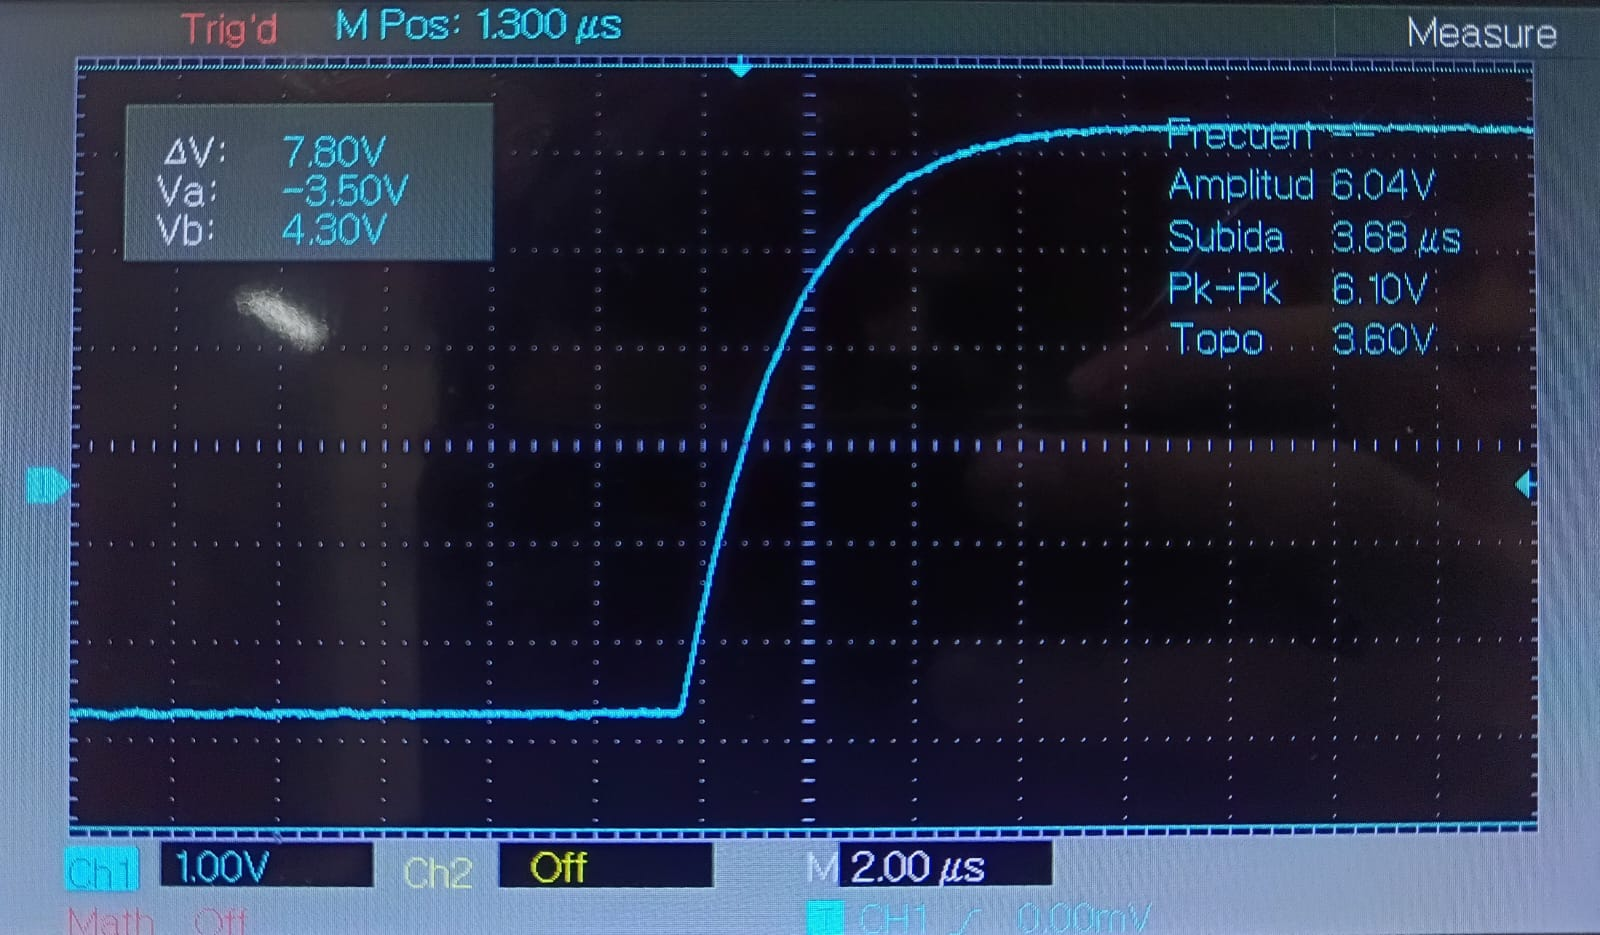
\includegraphics[width=1\textwidth]{Imagenes/tcLA.jpeg}
        \caption{Lazo Abierto}
        \label{fig:tcLA}
    \end{subfigure}
    \hfill
    \begin{subfigure}[b]{0.54\textwidth}
        \centering
            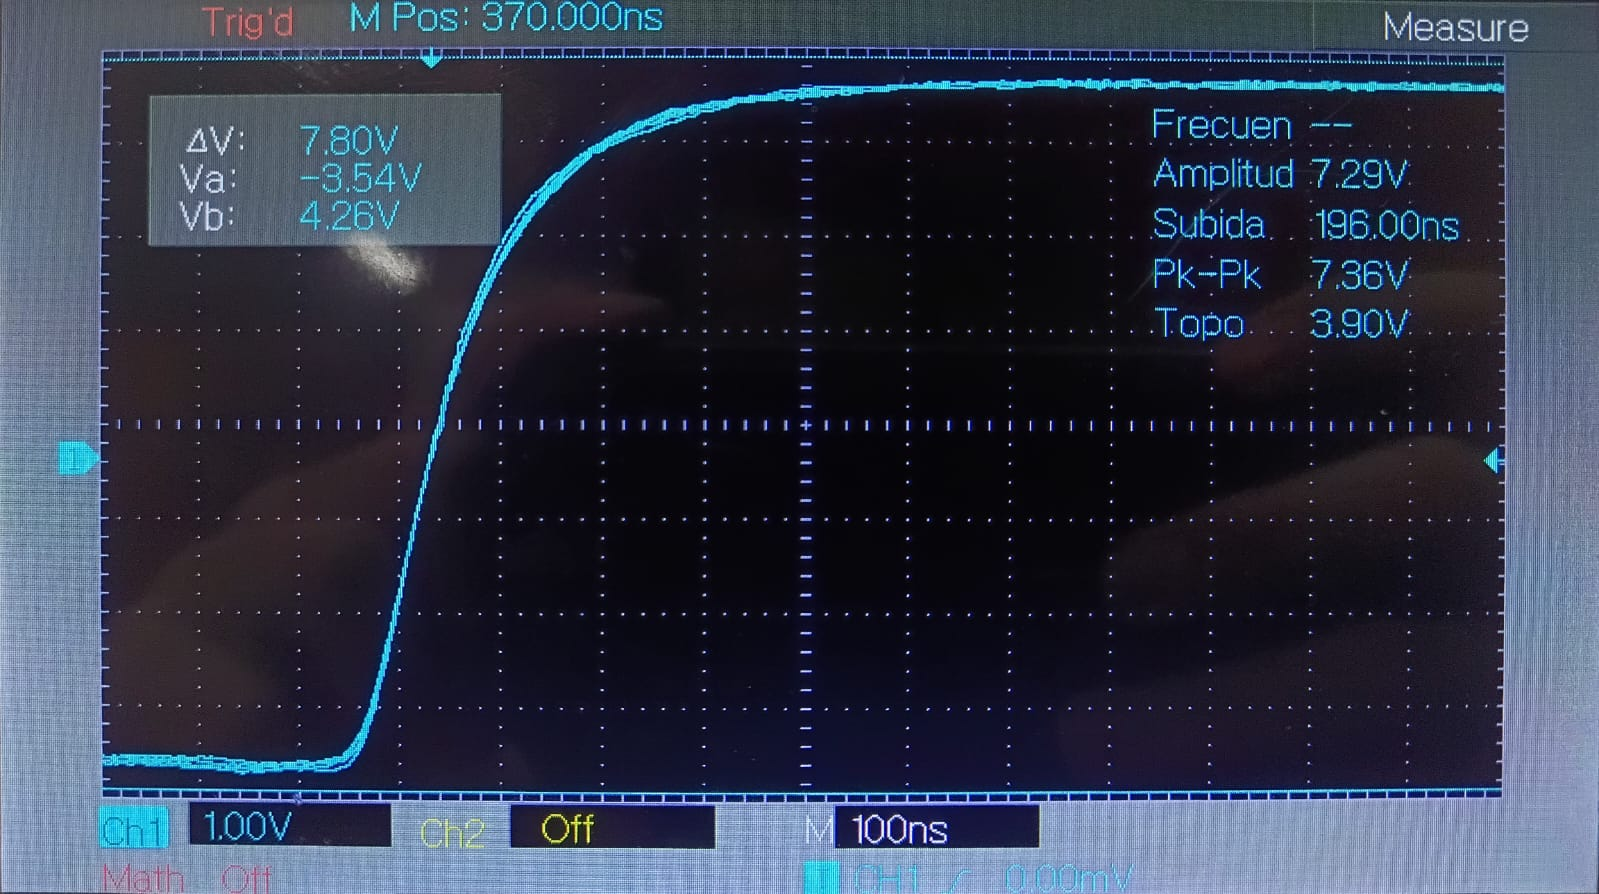
\includegraphics[width=1\textwidth]{Imagenes/tcLC.jpeg}
        \caption{Lazo Cerrado}
        \label{fig:tcLC}
    \end{subfigure}
    \caption{Flancos ascendente y tiempos de subida para cada configuración}
    \label{fig:tc}
    \end{center}
\end{figure}

Los valores obtenidos en cada caso fueron:

\begin{equation*}
    t_{c_{LA}} = 3,68 ~\mu s
    \hspace{1cm} y \hspace{1cm}
    t_{c_{LC}} = 196 ~ns
\end{equation*}

\subsubsection{Cálculos}

A partir de estos valores, se calculará el ancho de banda del amplificador. Pero antes de eso, se debe corroborar que el tiempo de subida, no sea comparable con el del osciloscopio, para lo cual se debe averiguar el tiempo de subida de este último. Para esto se utilizará la ecuación \ref{eq:tc_osc}, expuesta en el Marco Teórico. 

Para este experimento se utilizó el osciloscopio digital de la marca UNI-T, modelo UTD2102CEX. El ancho de banda de este osciloscopio es de 100 MHz.

\begin{equation*}
    t_{c_{osc}} = \cfrac{0.35}{AB_{osc}}
    \hspace{5mm} \Longrightarrow \hspace{5mm}
    t_{c_{osc}} = \cfrac{0.35}{100 \cdot 10^6 Hz} = 3.5 ns
\end{equation*}

Para el primer caso, amplificador a lazo abierto, el tiempo de crecimiento es mucho mayor que el recién calculado, por lo que no hace falta realizar la corrección. Además, del experimento anterior conocemos que este modo presenta una respuesta con caída exponencial, por lo que el \textit{k} valdrá 0,35. Partiendo de la ecuación \ref{eq:ABtc}, se tiene:

\begin{equation*}
    AB_{LA} = \frac{k}{t_{c_{LA}}} = \frac{0.35}{3.68 \cdot 10^{-6} [s]} = 95.109 kHz
\end{equation*}

Se aprecia que el ancho de banda obtenido, se aproxima al ancho de banda obtenido en el experimento anterior para este modo del amplificador.

Para el caso del amplificador realimentado, se tiene un tiempo de crecimiento bastante menor, el cual si puede llegar a verse afectado por el del osciloscopio. Por lo que aquí si se aplicará la ecuación de corrección (ecuación \ref{eq:correc}).

\begin{equation*}
     t_{c_{LC_{corr}}} = \sqrt{[t_{c_{LC}}]^2 + [t_{c_{osc}}]^2} = \sqrt{[196 \cdot 10^{-9}]^2 + [3.5 \cdot 10^{-9}]^2} = 196.03 ns
\end{equation*}

Finalmente, a partir de este valor y de los resultados del ejercicio anterior que demuestran que la respuesta tiene nuevamente una caída exponencial (k = 0,35), se calcula el ancho de banda del amplificador a lazo cerrado:

\begin{equation*}
    AB_{LC} = \frac{k}{t_{c_{LC_{corr}}}} = \frac{0.35}{196.03 \cdot 10^{-9} [s]} = 1.785 MHz
\end{equation*}

En este caso también se verifica que el cálculo se aproxima bastante a las mediciones de la experiencia anterior, por lo que se puede asumir que esta correctamente planteado.


\newpage
\section{Conclusión}
Con el presente trabajo se pudo aprender a como medir las impedancias y el ancho de banda de los amplificadores correctamente, parámetros muy importante para nuestra carrera. Además de medir lo efectos que tiene sobre estos parámetros la realimentación negativa.
Se pudo observar que, la realimentación negativa, aumenta el ancho de banda del amplificador a costa de reducir la ganancia. La realimentación negativa, además de tener un efecto sobre la respuesta en frecuencia, afecta las impedancias tanto de entrada como de salida. La impedancia de entrada aumentara, incrementando la ganancia en potencia del amplificador. Recordando la ecuación \ref{eq:Exp4PotZ},$P_{dB}=GV_{dB}-10\log{\frac{Z_L}{Z_e}}$ el efecto del segundo termino (correspondiente a las impedancias) tendrá un mayor efecto, aumentando la ganancia. Claro esto solo si tenemos en cuenta el efecto que tienen las resistencias y despreciando la perdida de ganancia en tensión. En cuanto a la transferencia de potencia, la disminución de la impedancia de salida no involucra una mayor potencia sobre la carga. Ahora, en el caso de la impedancia de entrada es de esperar que aumente la resistencia al ser una realimentación del tipo comparación de tensiones en serie.

Se aprendió a utilizar la escala de decibelios en el multimetro y como calibrarlo.
El usar un multimetro con escala en decibelios te da muchas ventajas que simplifican la experimentación, algunas de estas son:
\begin{itemize}
    \item Facilidad en el calculo, ya que la ganancia se obtiene realizando directamente la diferencia entre los valores de entrada y de salida, permitiendo observar fácilmente si nuestro amplificador magnifica, atenúa o no amplifica la señal de entrada.
    \item Permite visualizar de manera cómoda la variación de la ganancia en función de factores que poseen un amplio rango de variación.
    \item Al medir algún parámetro (potencia o tensión), el uso de escalas en decibeles permite visualizar de manera rápida y directa la magnitud medida. 
    \item El decibel se calcula en una escala logarítmica que permite la especificación del rendimiento a través de un amplio rango de voltaje/potencia.
\end{itemize}

En caso de que se cambie la escala,(respecto a el rango de $3V$)de un multimetro analógico al medir en decibelios, se debe aplicar un factor de corrección para las mediciones:
\begin{equation}
    dBu=dBu'+\log{\frac{Vr_1}{Vr_0}}
\end{equation}
Siendo $dBu'$ el valor medido por el multimetro, $Vr_0$ el valor de la escala inicial (en nuestro caso $3V$) y $Vr_1$ el valor de la nueva escala.





\vspace{1cm}
\section{Bibliografía}
\begin{itemize}
   %\item \url{}
    \item \url{https://www.studocu.com/es-ar/document/universidad-tecnologica-nacional/medidas-electronicas-i/ganz-univo-elektronik-01-sm/53094434}
\end{itemize}

\newpage

\section{Anexo}

\label{sec:Información Instrumentos}


\begin{table}[h!]
    \centering
    \scalebox{1}{
    \begin{tabular}{|c|c|c|}
    \hline
         Range & Resolution & Accuracy \\
    \hline
         600.0 $\Omega$ & 0.1 $\Omega$ & $\pm$(0.8$\%$ + 5) \\
    \hline
        6.000 k$\Omega$ & 0.001 k$\Omega$ & \multirow{4}{*}{$\pm$(0.8$\%$ + 3)} \\
    \cline{1-2}
        60.00 k$\Omega$ & 0.01 k$\Omega$ &\\    
    \cline{1-2}
        600.0 k$\Omega$ & 0.1 k$\Omega$ &\\
    \cline{1-2}
        6.000 M$\Omega$ & 0.001 M$\Omega$ &  \\
    \hline
        60 M$\Omega$ & 0.01 M$\Omega$ & $\pm$(3.0$\%$ + 10) \\
    \hline
    
        \end{tabular}}
        \def\tablename{Tabla} 
        \caption{Tabla de Precisión del Ohmetro del tester UT890C}
        \label{tab:R_UT890C}
\end{table}





\begin{table}[h!]
    \centering
    \scalebox{1}{
    \begin{tabular}{|c|c|c|}
    \hline
         Range & Accuracy \\
    \hline
    \multicolumn{2}{|c|}{50Hz-60Hz}\\
    \hline
         400mV-4V & \multirow{3}{*}{$\pm$(0.5$\%$ + 3)} \\
         40V-400V& \\
         750V& \\
    \hline
      \multicolumn{2}{|c|}{40Hz-1kHz}\\
    \hline
         400mV & $\pm$(0.8$\%$+3)\\
         \hline
         4V-40V&\multirow{2}{*}{$\pm$(0.8$\%$ + 4)} \\
         40V-400V& \\
         \hline
         750V& $\pm$(1.0$\%$+4)\\
    \hline
      \multicolumn{2}{|c|}{1KHz-50kHz}\\
    \hline
         400mV & $\pm$(1$\%$+3)\\
         \hline
         4V-40V&\multirow{2}{*}{$\pm$(1$\%$ + 4)} \\
         40V-400V& \\
         \hline
         750V& $\pm$(3.0$\%$+6)\\
    \hline
      \multicolumn{2}{|c|}{5KHz-20kHz}\\
    \hline
         400mV & $\pm$(1.5$\%$+6)\\
         \hline
         4V-40V&\multirow{2}{*}{$\pm$(1.8$\%$ + 6)} \\
         40V-400V& \\
         \hline
         750V& Unspec'd\\
    \hline
      \multicolumn{2}{|c|}{5KHz-20kHz}\\
    \hline
         400mV & $\pm$(2.5$\%$+6)\\
    \hline
        \end{tabular}}
        \def\tablename{Tabla} 
        \caption{Tabla de Precisión del Voltímetro del tester BM837RS}
        \label{tab:ACV_BM837RS}
\end{table}




\end{document}